% For instructions, 
\documentclass[ reprint, amsmath,amssymb, aps]{revtex4-2}

%\usepackage[norsk]{babel}
%Uncomment this if you want to write in Norwegian
\usepackage{listings}
\usepackage{graphicx}% Include figure files
\usepackage{dcolumn}% Align table columns on decimal point
\usepackage{bm}% bold math
\usepackage{hyperref}% add hypertext capabilities
\usepackage{booktabs}
\usepackage{float}

\begin{document}

\title{Modellering av "Temperfect mug"}
%In a multipart project you may find a title that covers the common aspects of what you present


\author{Henrik Modahl Breitenstein}



\date{\today}

\begin{abstract}
Vi ser på to isolerende kopper hvor den en har et faseskiftende matrielet inne i seg. Vi prøver å modellere varmetapet til koppen med det faseskiftende materialet med å bruke varmekapasiteten fra einsteinkrystall modell. Modellen passer bra, men har også noen overganger hvor det ikke stemmer overens.
\end{abstract}

\maketitle

%\onecolumngrid

\section{Introduction}
Det å kunne bevare varme har alltid vært viktig. For å kunne teste løsninger teoretisk så prøver vi å finne en forenklet modell som passer bra til systemet. Vi skal se på en isolerende kopp laget av Joeveo. De sier koppen ekstraherer den riktige mengden varme fra kaffen eller teen din, og bruker den varmen til å opprettholde drikken på den perfekte temperaturen i en lengre periode. Koppen gjør dette ved å bruke et materiele med faseovergang ved temperaturene nylagd kaffe og te er på til vanlig , i tillegg til å bruke luftsisolasjon. I en kopp uten isolasjon, så vil temperaturen endre seg ifølge varmefluksen ut gjennom luften:

\begin{equation}
\label{heatflux}
AJ_q = \frac{\mathrm{d}Q}{\mathrm{d}t} = mc_v\frac{\mathrm{d}T}{\mathrm{d}t}
\end{equation}  

Hvor $A$ er arealet, $Q$ er varmen, $m$ er massen og $c_v$ er den spesifikke varmekapasiten til vannet. Varmefluksen gjennom veggen av koppen vil være:

\begin{equation}
\label{veggtap}
\vec{J_q} = - \lambda \nabla{T}
\end{equation}

Hvor $T$ er temperaturen og $\lambda$ er den termiske konduktiviteten. Ved kun tap gjennom veggene så kan vi skrive:

\begin{equation}
\label{kunvegg}
\frac{\Delta{T}}{\Delta{T_0}} = e^{-t/\tau} 
\end{equation}

Hvor $\Delta{T}$ er forholdet mellom temperaturen til vannet og luften rundt, og $\tau$ er en tidskonstant. For å finne et uttrykk for $\tau$ så  ser vi på utledelsen av \ref{kunvegg}. Ved å sette fluksen fra \ref{heatflux} og \ref{veggtap} lik hverandnre så ender vi opp med

$$\frac{\mathrm{d} \Delta T}{\mathrm{d}t} + \frac{\lambda A}{m c_v} \Delta{T} = 0 \; ,$$

Hvor da $\Delta T = T - T_a$. Tar integralet og får at

$$\ln{\Delta T} - \ln{\Delta T_0} = -\frac{\lambda A}{c_v m} t$$

Som gir oss \ref{kunvegg}, hvor

\begin{equation}
\label{tau}
\tau = \frac{mc_v}{\lambda A}
\end{equation}

I likningen oven for så kan man enten tenke seg en konstant varmekapasitet eller en som endrer seg med temperaturen. For å se på det sistnevnte så skal vi bruke modellen for en einsteinkrystall med $N$ oscilatorer og $q$ energikvanta. Man vil da kunne skrive at multiplisiteten $\Omega$

\begin{equation}
\label{Ohm}
\Omega \approx \left ( \frac{q+N}{q}\right )^q \left ( \frac{q+N}{N}\right )^N \; .
\end{equation} 

Med det kan vise følgende analytiske uttrykk

\begin{equation}
\label{S}
 S = (q+N)\ln{q+N} - q \ln{q} - N\ln{N} \; ,
\end{equation}


hvor $S$ er entropien til systemet.

\begin{equation}
\label{T}
T' = \frac{\epsilon}{\ln{\frac{q+N}{q}}} \; ,
\end{equation}

hvor $T' = \frac{T \epsilon}{k_B}$ der $T$ er temperaturen, $\epsilon$ er energikvanta og $k_B$ er boltzmannskonstant.

\begin{equation}
\label{C}
C_v(T') = \frac{e^{1/T'}}{(e^{1/T'} - 1)^2} \; ,
\end{equation} 

hvor $C_v$ er varmekapasiteten til systemet.

Ved å kombinere de to systemene skal vi se om vi kan finne en modell som passer til 'Temperfect mug' sitt varmetap.
\clearpage
\onecolumngrid

\section{Results and discussion}


Varmetapet til Bodum-koppen og 'Temperfect mug' er skissert i \ref{varmetapRep}


\begin{figure}[ht]
\centering
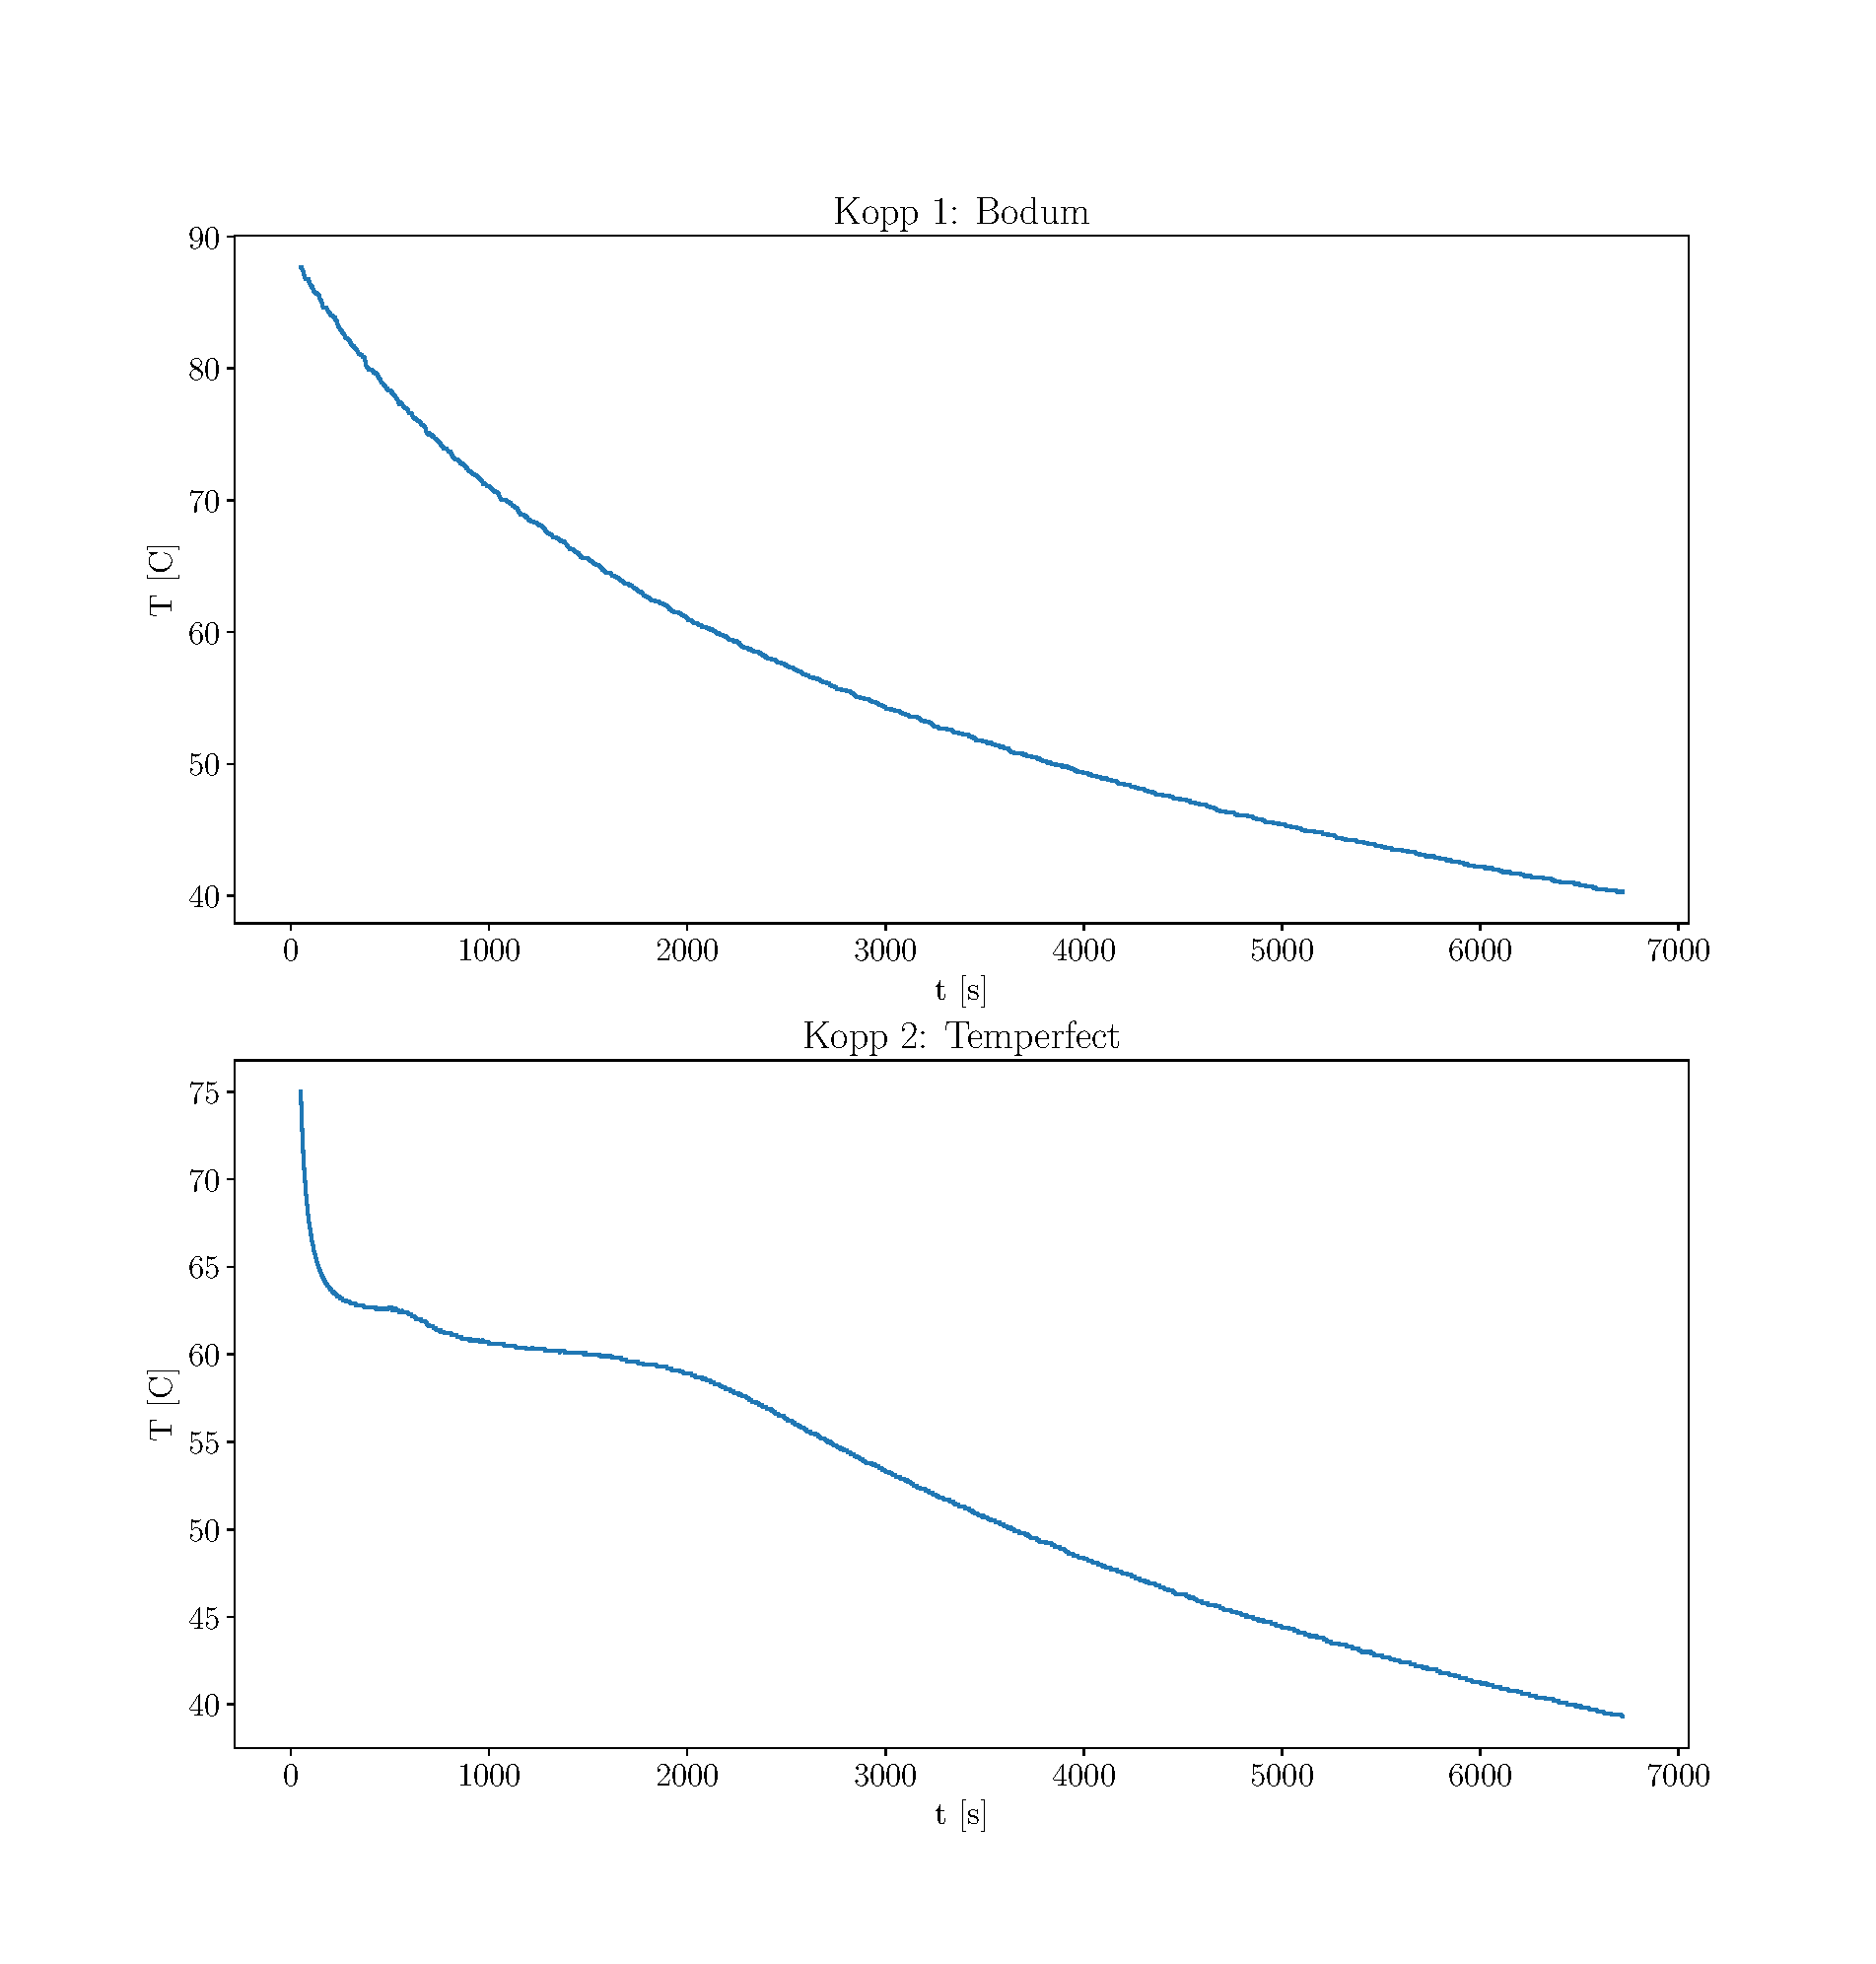
\includegraphics[scale=0.5]{tempkopp.pdf}
\caption{Temperaturen, målt i grader celcius, til vannet i koppene etter tiden $t$.}
\label{varmetapRep}
\end{figure}

\twocolumngrid
\clearpage
kopp 1, og senere kopp 2, ser ut til å følge et eksponentsiell forfall, som forventet. Vi ser først på kopp 1, den vanlige thermosen. Om vi antar det kun er fra veggene så skal den følge likningen \ref{kunvegg}. Vi finner tidskonstanten ved at 

$$\frac{\Delta T}{\Delta T_0} = e^{-1} \Rightarrow \tau = t$$

Og får skissen \ref{plotm1Rep}

\begin{figure}
\centering
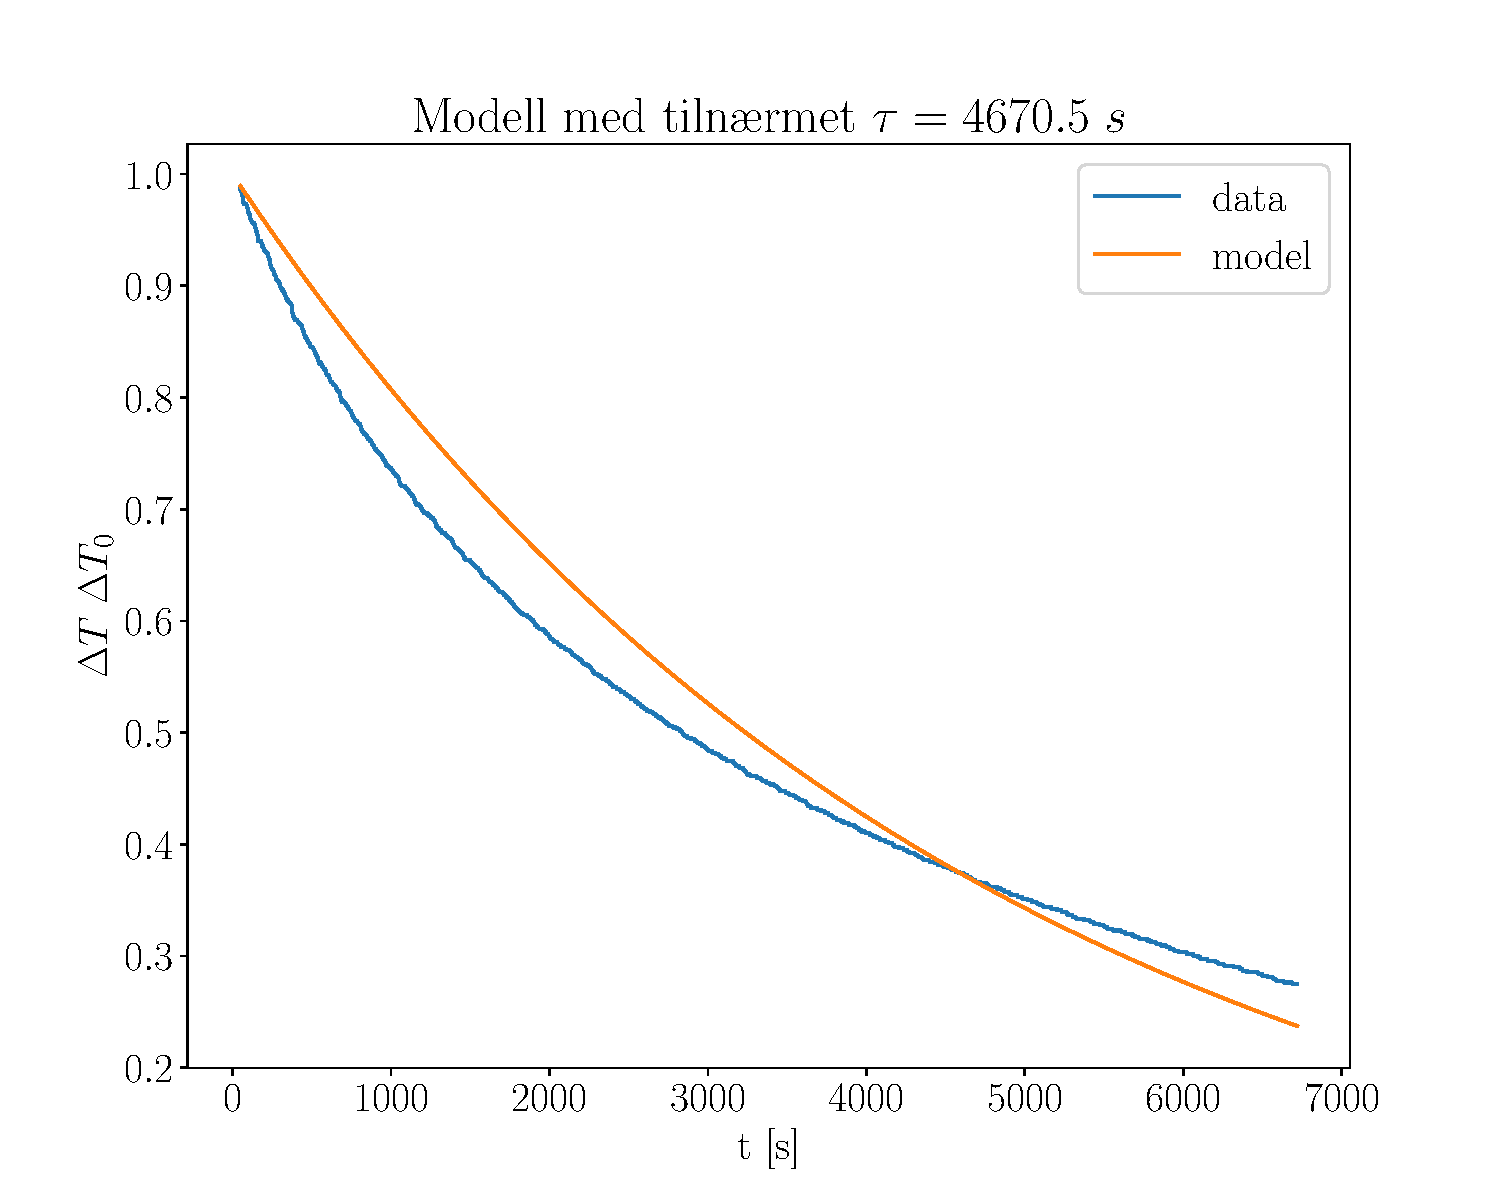
\includegraphics[scale=0.35]{modellttau.pdf}
\caption{Plot av modell sammen med data til den normale koppen. Her er $\tau = 4670.5 \; s$.}
\label{plotm1Rep}
\end{figure}

Vi ser at modellen passer ganske godt, men ikke helt perfekt. Vi kunne tenkt oss at å ha at den mister varme både gjennom veggen og fra toppen av koppen, men det vil bare gi en til proporsjonalitet med temperaturforskjellen, som vil allerede ligge i proporsjonalitetskonstanten i \ref{veggtap}. Modellen må også kunne gjøre rede for utflatingen i starten til grafen av varmetapet til kopp 2. Forkjellen mellom kopp 1 og 2 er stor i starten men blir like etter en stund, som vist i \ref{tempdifRep} 

\begin{figure}
\centering
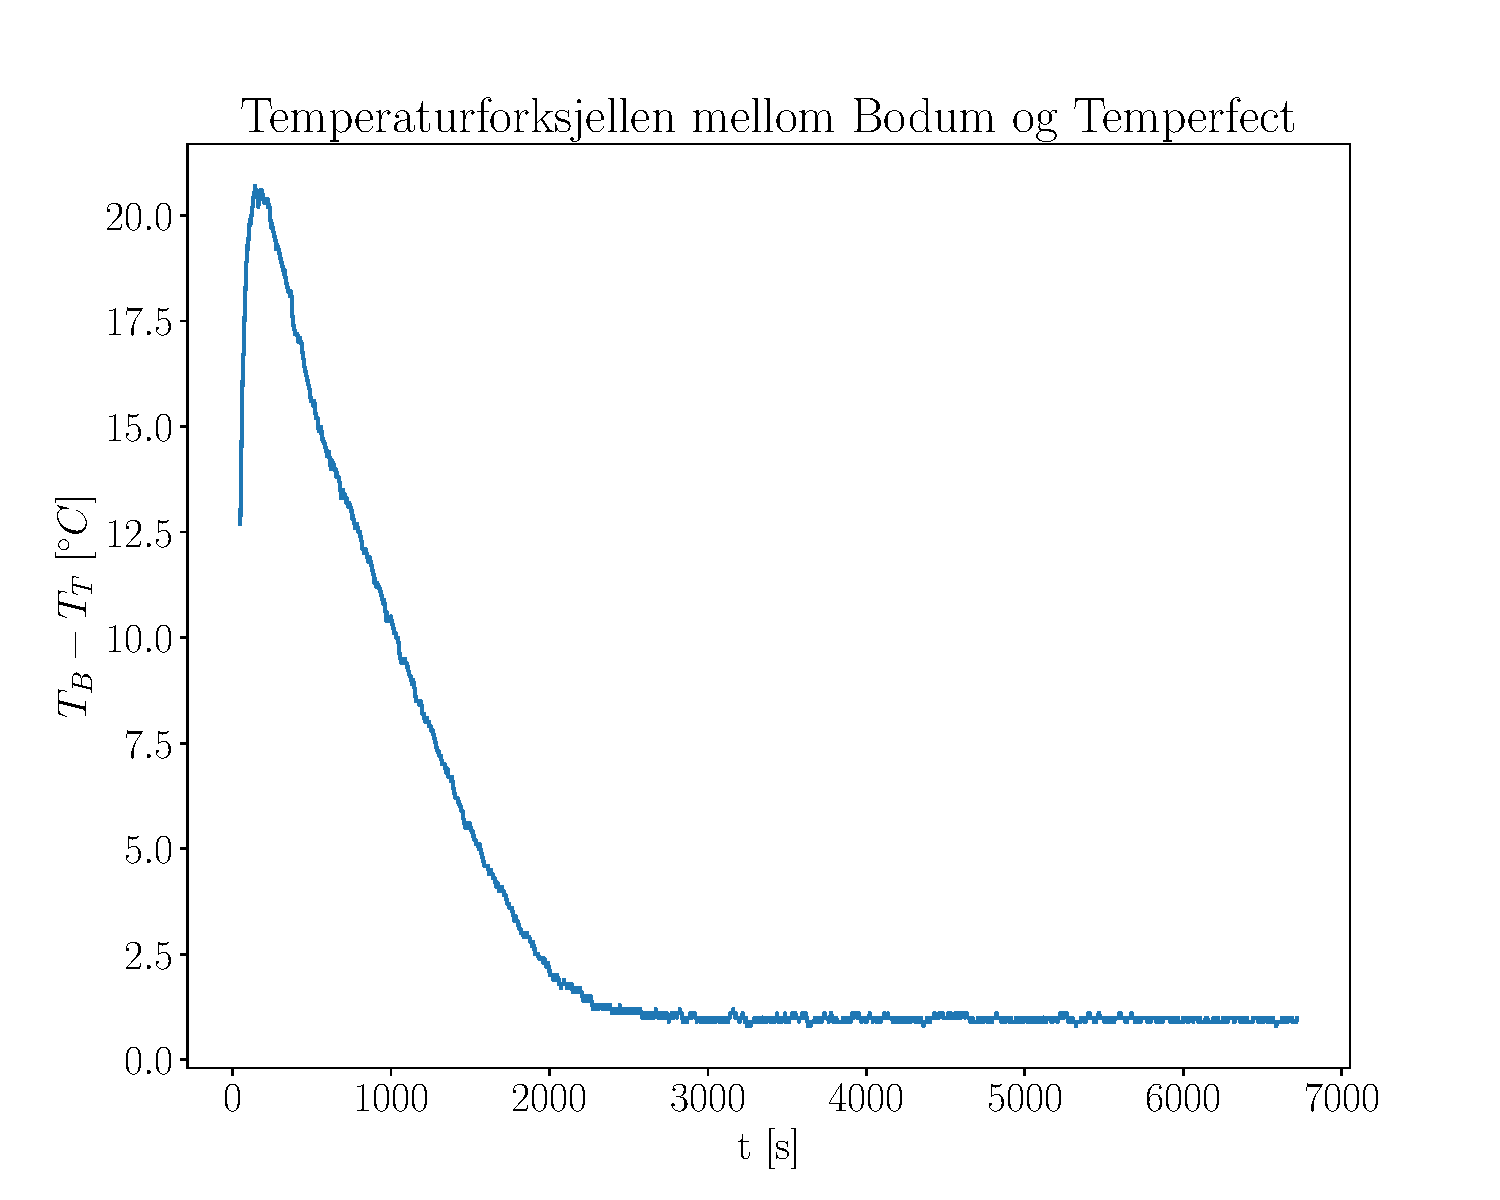
\includegraphics[scale=0.35]{tempzoomedout.pdf}
\caption{Temperaturforksjllen mellom Bodum-koppen og 'Temperfect mug'.}
\label{tempdifRep}
\end{figure}

Som er fordi 'Temperfect mug' har et faseskiftende materiale og om vi ser på grafen \ref{varmetapRep}, så ser vi at grafen til 'Temperfect mug' flater ut ved ca. 63 grader celsius, og faseskiftet er når den går videre ned, så vi kan anta:

$$T_m \approx 61 \; ^{\circ}C$$

Der $T_m$ er smeltepunktet til materialet. Om vi ser på posisjonene på grafen, så ser vi at den første flate biten varer fra $200 \; s$ til $600 \;s$, som ville vært når materielet smelter. Den andre flate biten, når materielt krystaliseres, er fra $600 \; s$ til $2000 \; s$. Så vi den tar opp varme i en kortere periode enn den gir ut varmen tilbake til vannet igjen. Den totale energien som den har lagret ved punktet hvor den er blitt flytende kan vi finne ved å se på forskjellen. 

Om vi regner med at all energien som vannet mister er det som blir gitt til det faseskiftende materialet. Så var det omtrent $18.1 \; ^{\circ}C$ av vannet som ble tatt opp av det faseskiftende materialet. Hvor mye energi dette er avhenger av den spesifikke varme kapasiteten og massen til vannet:

$$Q = T m c_v.$$
$$Q = 18.1 \; K \cdot 0.3 \; kg \cdot 4205 \; K^{-1}\; kg^{-1} \; J $$
$$Q \approx 22.8 \; kJ$$

Om vi tenker oss at materielts varmekapasitetsforholdet endrer seg fra $\frac{C_{V, c}}{C_{V, w}} = 0.1$ til $\frac{C_{V, c}}{C_{V, w}} = 4$ så kan vi prøve å modellere varmetapet som en abrupt endring i varmekapasiteten til den faseskiftende materialet ved $T_m$, vi kan kalle det for en naive modell. Med den naive modellen så vil vi ha to eksponentsielle forfallsfunksjoner hvor

$$\tau_1 = 0.1 \tau_0$$
$$\tau_2 = 4 \tau_0$$

Om vi bruker $ \tau_0 = \frac{4670.5}{4}$ så får vi at den følger Bodum-koppens kurve etter skiftet. Det vil gi oss en rask reduksjon fulgt av en utstrakt reduksjon, som vist i skissen \ref{plot2tauRep}.

\begin{figure}
\centering
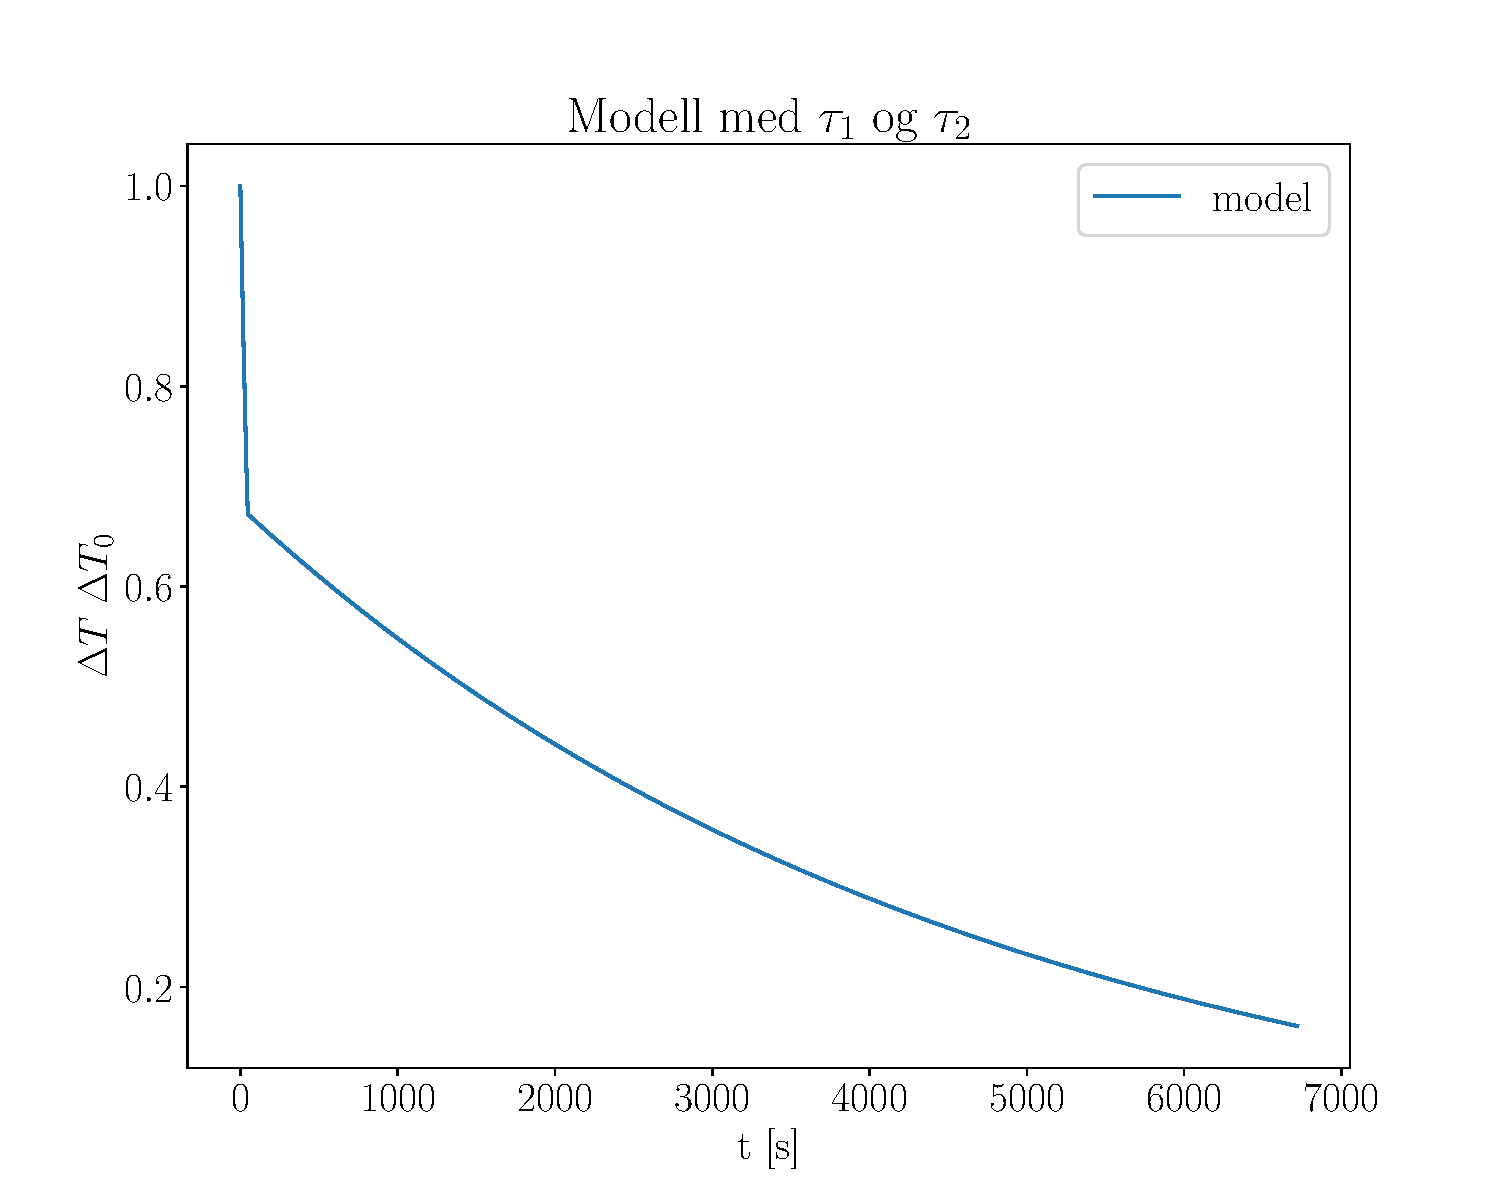
\includegraphics[scale=0.35]{2tauplot.pdf}
\caption{Skisse av hvordan den naive modellen for varmakapasitansforholdet vil se ut som en modell for 'Temperfect mug'.}
\label{plot2tauRep}
\end{figure}

Den modellen passer ikke så bra siden vi ikke har med den delen hvor temperaturkurven flater ut, men bedre enn uten skifte i varmekapasiteten. For ¨forbedre modellen så kan vi prøve å bruke en kontinuerlig endring av varmekapasiteten. En modell for varmekapasiteten har vi i \ref{C}. Den oppfører seg som vist i \ref{VanalytiskRep}

\begin{figure}
\centering
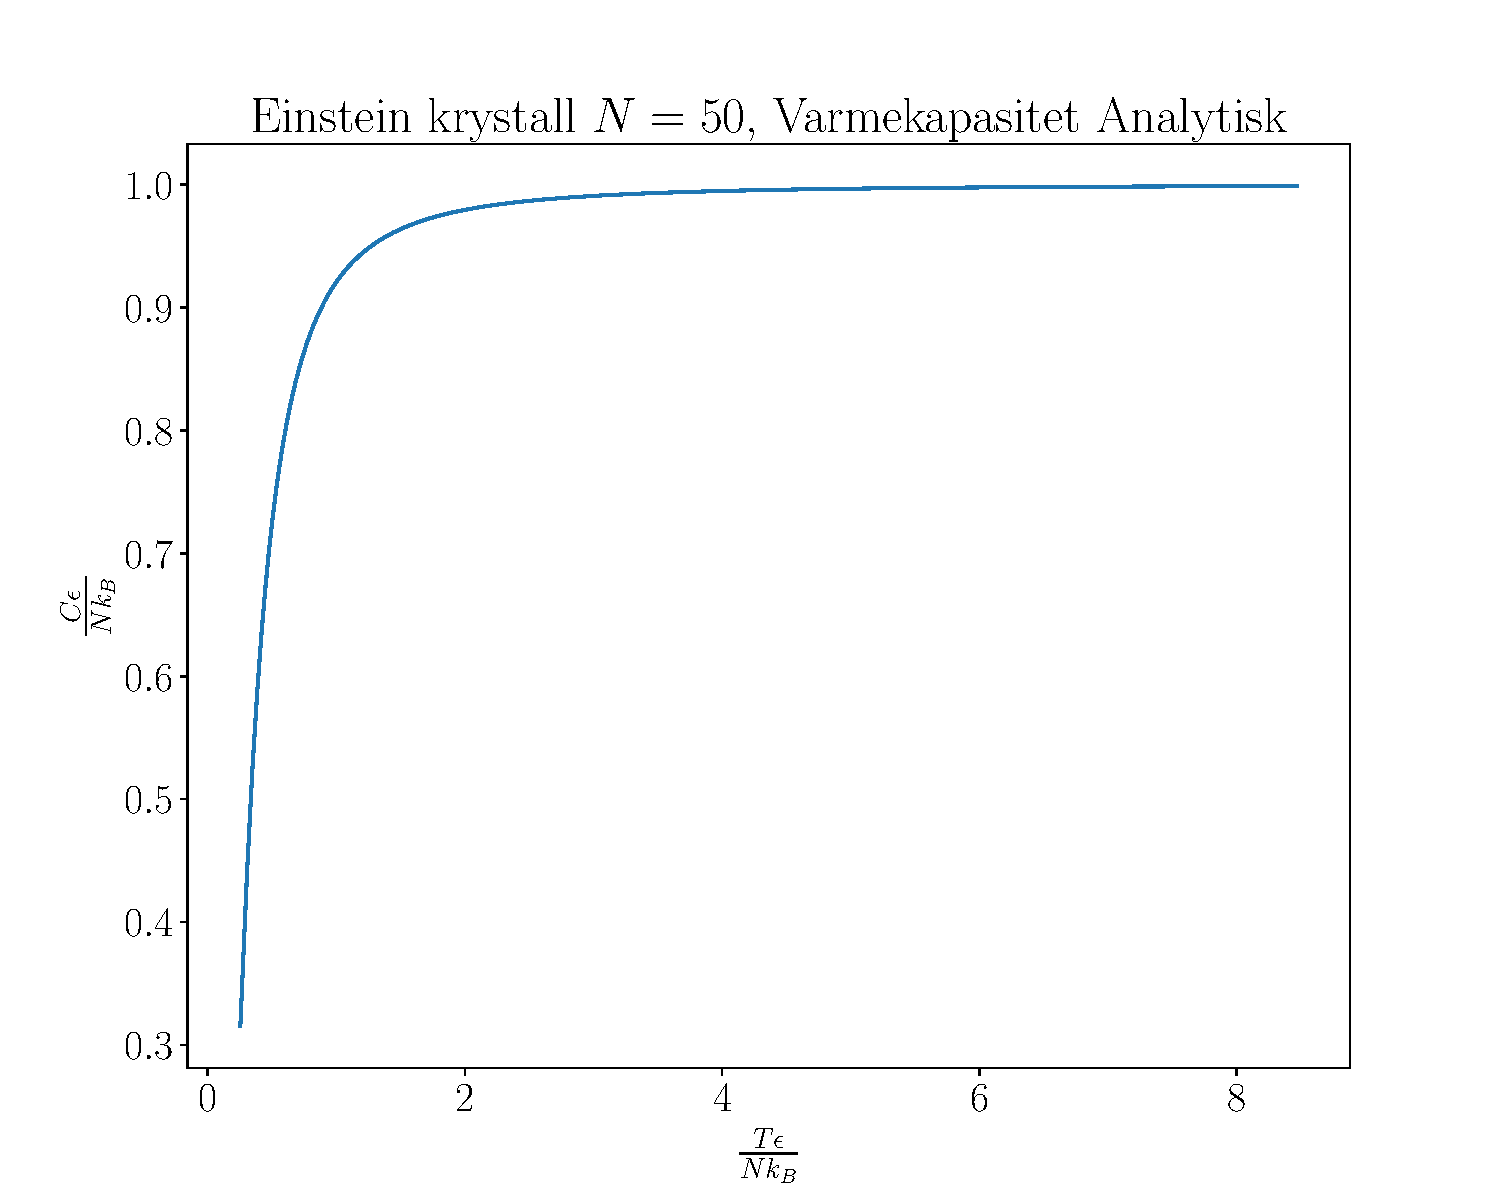
\includegraphics[scale=0.35]{Vanalytisk.pdf}
\caption{Den analytiske varmekapasiteten for einsteinkrystall.}
\label{VanalytiskRep}
\end{figure}

Vi prøver å bruke \ref{VanalytiskRep} som en modell for varmekapsitetsforholdet mellom vannet og veggen i 'Temperfect mug'. Vi har da at

$$\tau = C_V(T')\tau_0 \; .$$

Vi vil at modellen skal følge de to krumningene til 'Temperfect mug'. Vi ønsker også å ha at den følger grafen til kopp 1 først etter omtrent $59 ^{\circ}C$.

Ved å prøve fram til riktige verdier så fikk vi skissen \ref{epsTerm}.

\begin{figure}[H]
\centering
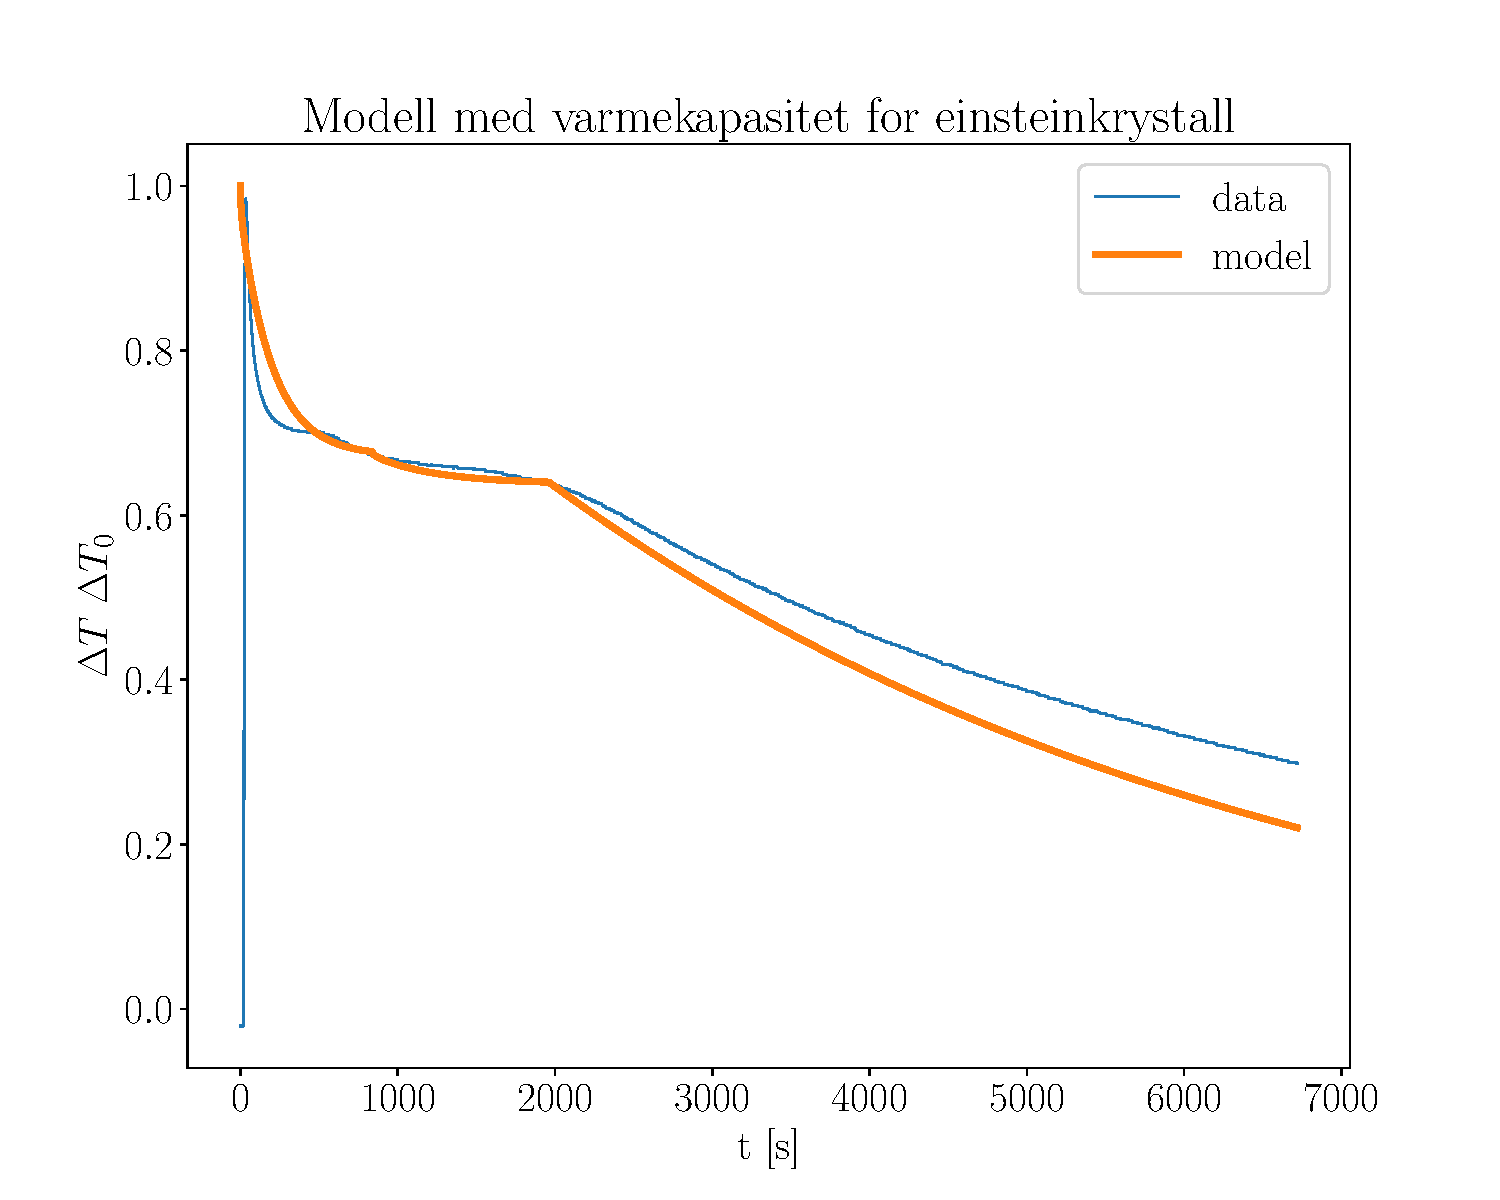
\includegraphics[scale=0.35]{modelleinstein.pdf}
\caption{Kombinert eisnteinkrystall modellens varmekapasitet med forholdet mellom vann og vegg i 'Temperfect mug'.}
\label{epsTerm}
\end{figure}

Vi ser at modellen har noen av de samme krumningene, men ikke overgangen mellom krumningene og overgangen til kurven grunnet varmetap til veggene av thermosen. For reproduserbarhet, så har vi lagt ved programmet som lager skissen, referer til metodedelen.
'clearpage
\onecolumngrid
\section{Methods}

For å skissere modellen med varmekapasieten fra einsteinkrystall modellen, så har vi gjort følgende:

\lstinputlisting[language=Python]{epsTerm.py}
\twocolumngrid
\section{Conclusion}

For 'Temperfect mug' så konkluderer vi med at å bruke einsteinkrystallmodellen til å modellere varmekapsiteten er en god metode, men har tydelige feil. Man får med en kontinuerlig skifte i varmekapasiteten, men ikke i overgangene mellom to faser. 


\bibliographystyle{unsrt}
\bibliography{Bibliography.bib}



\clearpage
\appendix

\section{Requested problems}
\onecolumngrid

\subsection*{Lag en skisse av varmetapet til det normale kruset.}

Lager en skisse av tempereaturene etter tiden $t$ i \ref{tempkopp}.

\begin{figure}
\centering
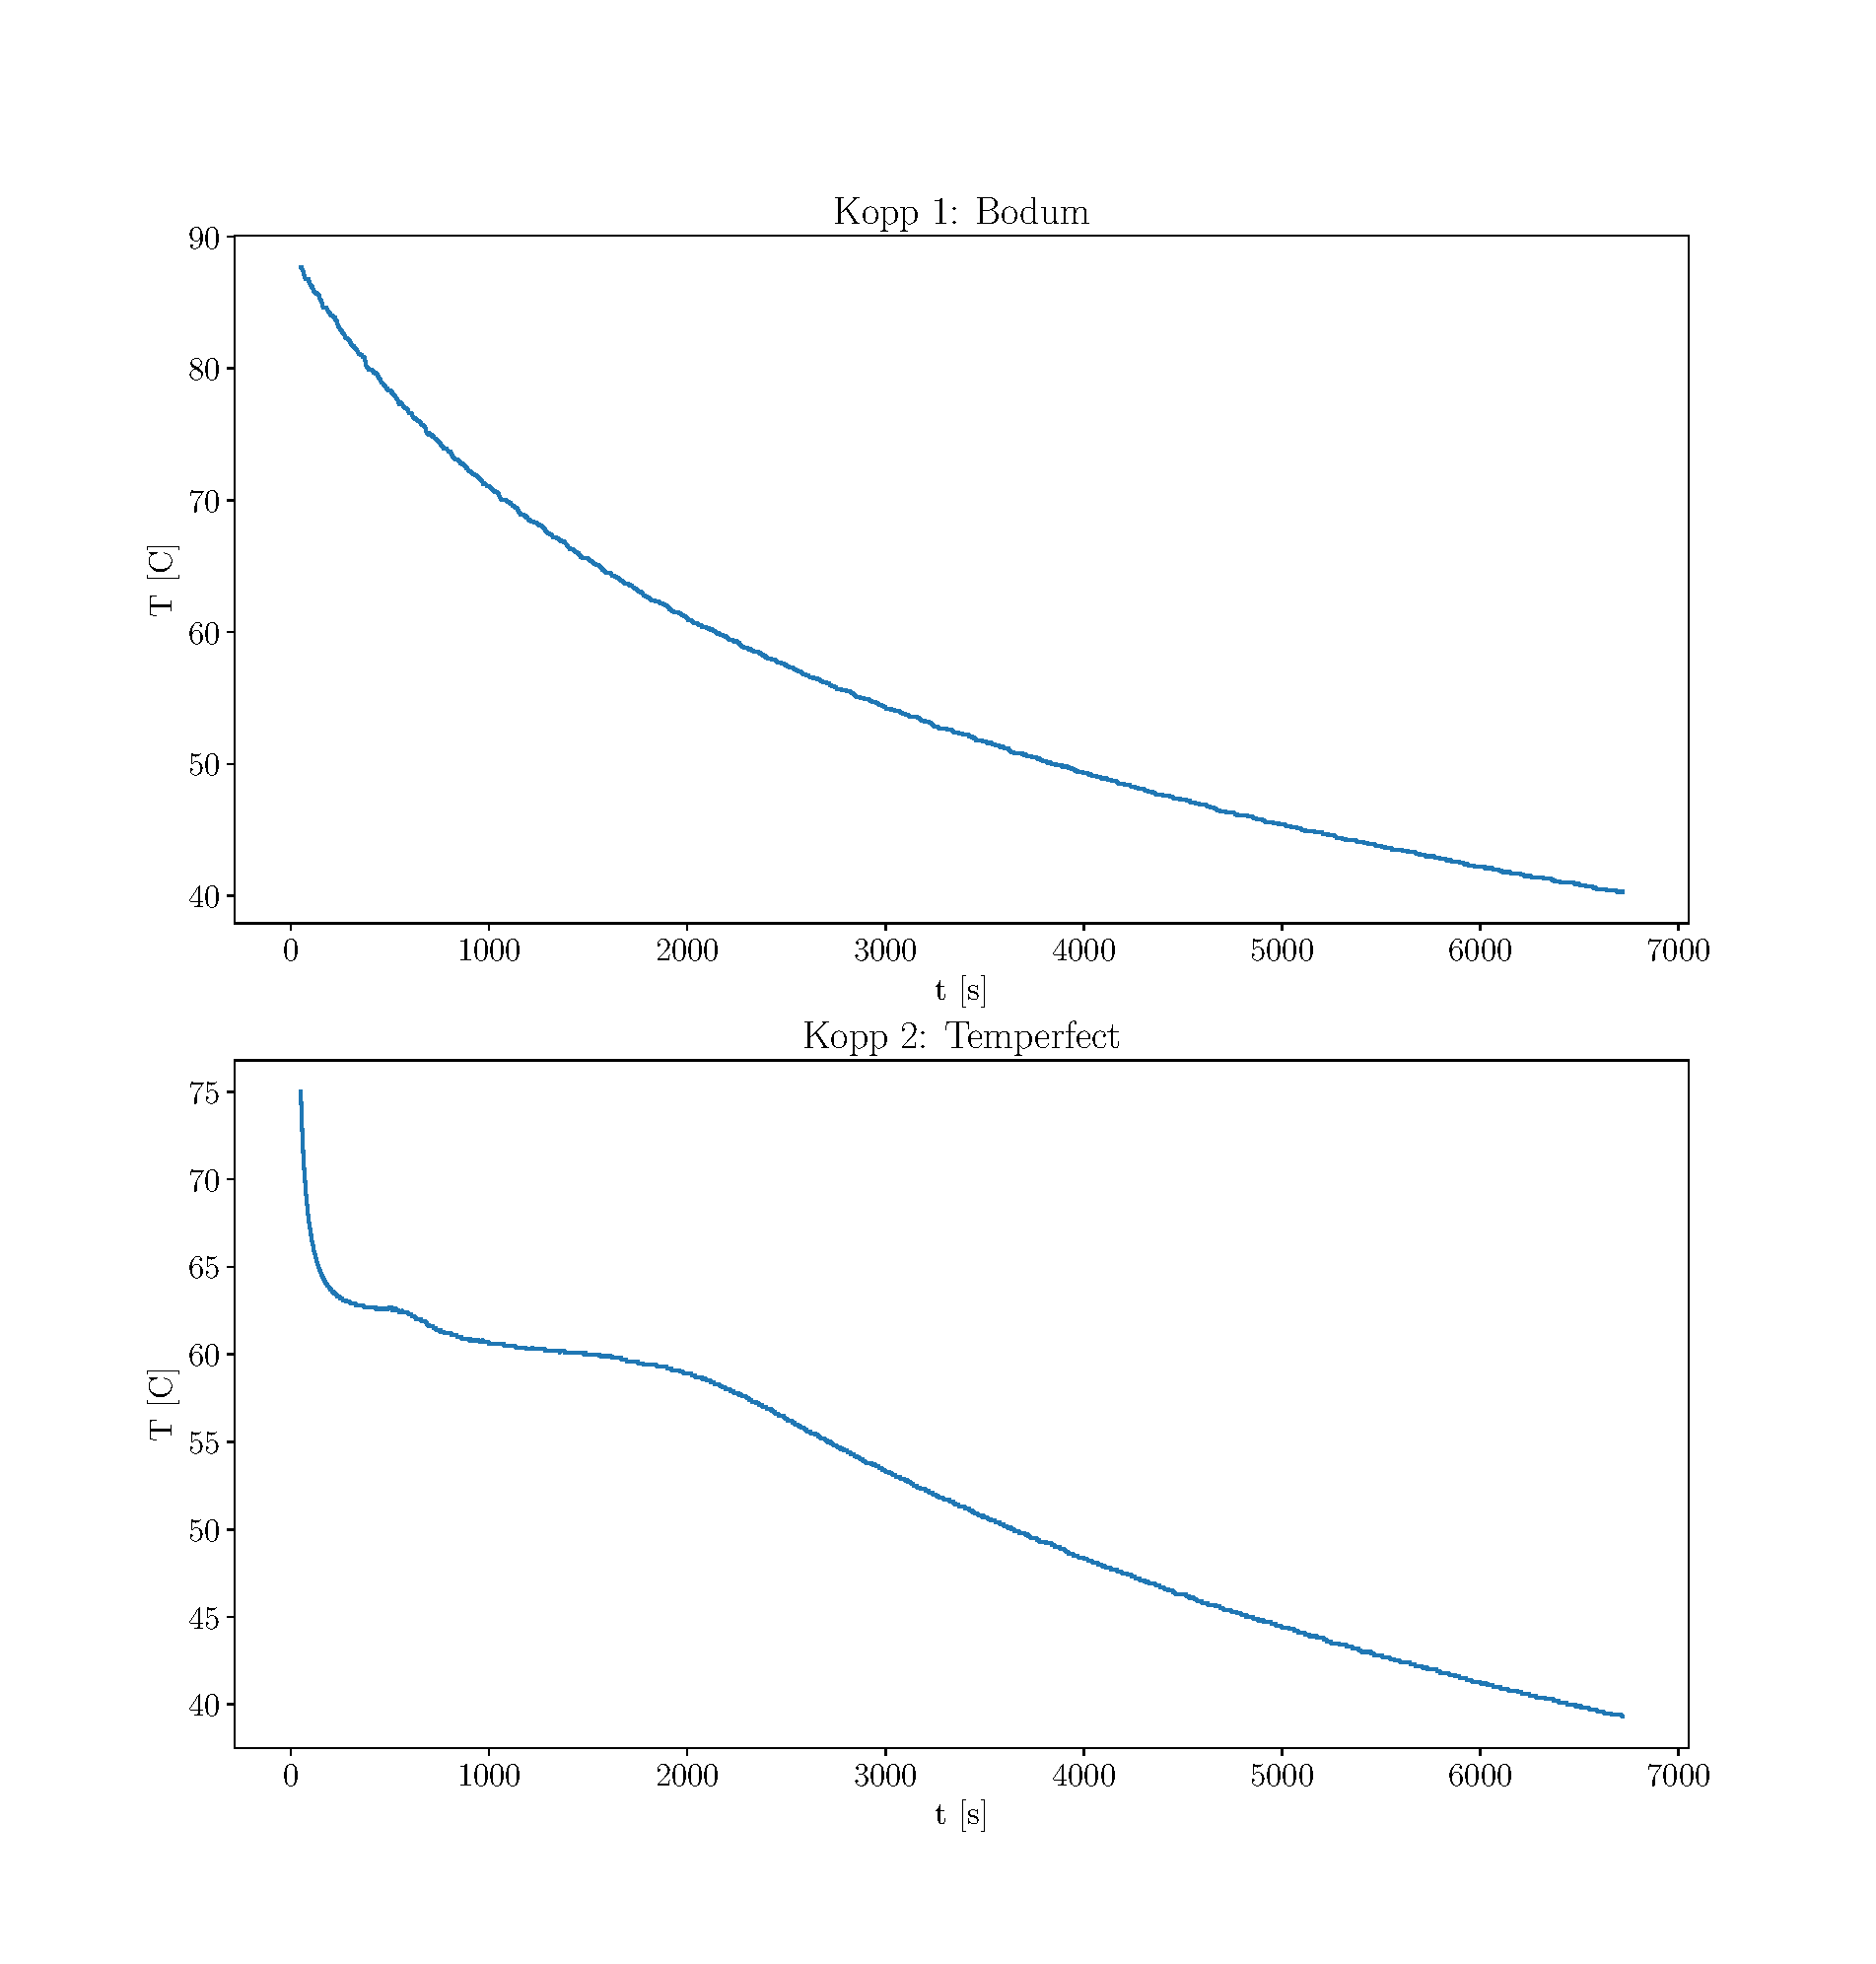
\includegraphics[scale=0.5]{tempkopp.pdf}
\caption{Temperaturen, målt i grader celcius, til vannet i koppene etter tiden $t$.}
\label{tempkopp}
\end{figure}
\twocolumngrid


\subsection*{Ved hjelp av skissen så burde du klare å finne et uttrykk for $\tau$.}

Fra \ref{kunvegg} så har vi at

$$\frac{\Delta T}{\Delta T_0} = e^{-1} \Rightarrow \tau = t$$

Finner en tilnærming for $\tau$ til Bodum-koppen og skisserer modellen opp mot data som er vist i \ref{plotm1}

\begin{figure}
\centering
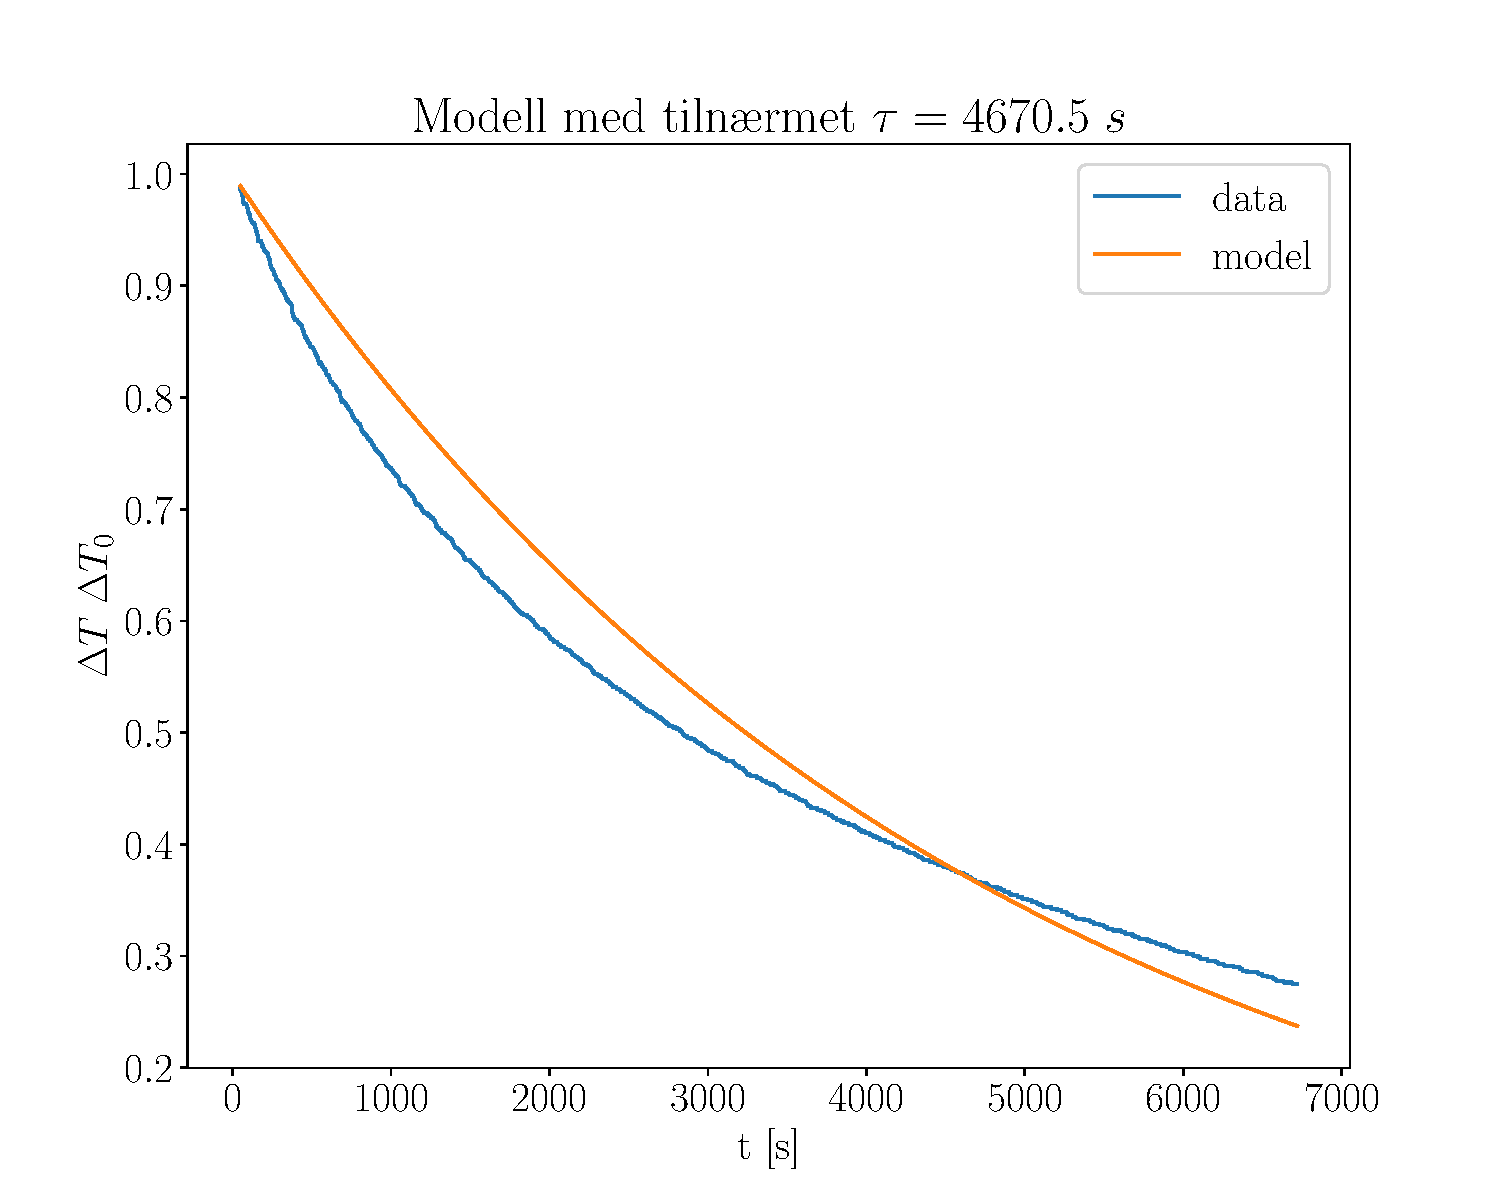
\includegraphics[scale=0.35]{modellttau.pdf}
\caption{Plot av modell sammen med data til den normale koppen. Her er $\tau = 4670.5 \; s$.}
\label{plotm1}
\end{figure}

\subsection*{Kan du gjøre modellen bedre med å ta med toppen av koppen som ikke er dekket til?}

Fra utregningen av \ref{kunvegg} så vil varmetapet fra den åpne toppen være en ekstra proporsjonalitet med temperaturforskjellen, så det vil kun endre hva konstanten $\tau$ representerer.

\subsection*{Hva er smeltepunktet til det faseskiftende materialet i 'Temperfect mmug'?}

Ser på grafen \ref{tempkopp} og ser at grafen til 'Temperfect mug' flater ut ved ca. 63 grader celsius, og faseskiftet r når den går videre ned, så tenker:

$$T_m \approx 61 \; ^{\circ}C$$

\subsection*{I hvilken periode smeltet materielt og i hvilken periode krystliserte den seg?}

Ser på posisjonene på grafen og ser at den første flate biten varer fra $200 \; s$ til $600 \;s$, som ville vært når materielet smelter. Den andre flate biten, når materielt krystaliseres, er fra $600 \; s$ til $2000 \; s$. 

\subsection*{Hvor mye varme ble lagret i det faseskiftende materialet.}

Om vi regner med at all energien som vannet mister er det som blir gitt til det faseskiftende materialet. Så var det omtrent $18.1 \; ^{\circ}C$ av vannet som ble tatt opp av det faseskiftende materialet. Hvor mye energi dette er avhenger av den spesifikke varme kapasiteten og massen til vannet:

$$Q = T m c_v.$$
$$Q = 18.1 \; K \cdot 0.3 \; kg \cdot 4205 \; K^{-1}\; kg^{-1} \; J $$
$$Q \approx 22.8 \; kJ$$

\subsection*{Er den naive modellen for faseskiftende materiale en bra modell for 'Temperfect mug'?}

Med den naive modellen så vil vi ha to eksponentsielle forfallsfunksjoner hvor

$$\tau_1 = 0.1 \tau_0$$
$$\tau_2 = 4 \tau_0$$

Om vi bruker $ \tau_0 = \frac{4670.5}{4}$ så får vi at den følger Bodum-koppens kurve etter skiftet. Det vil gi oss en rask reduksjon fulgt av en utstrakt reduksjon, som vist i skissen \ref{plot2tau}

\begin{figure}
\centering
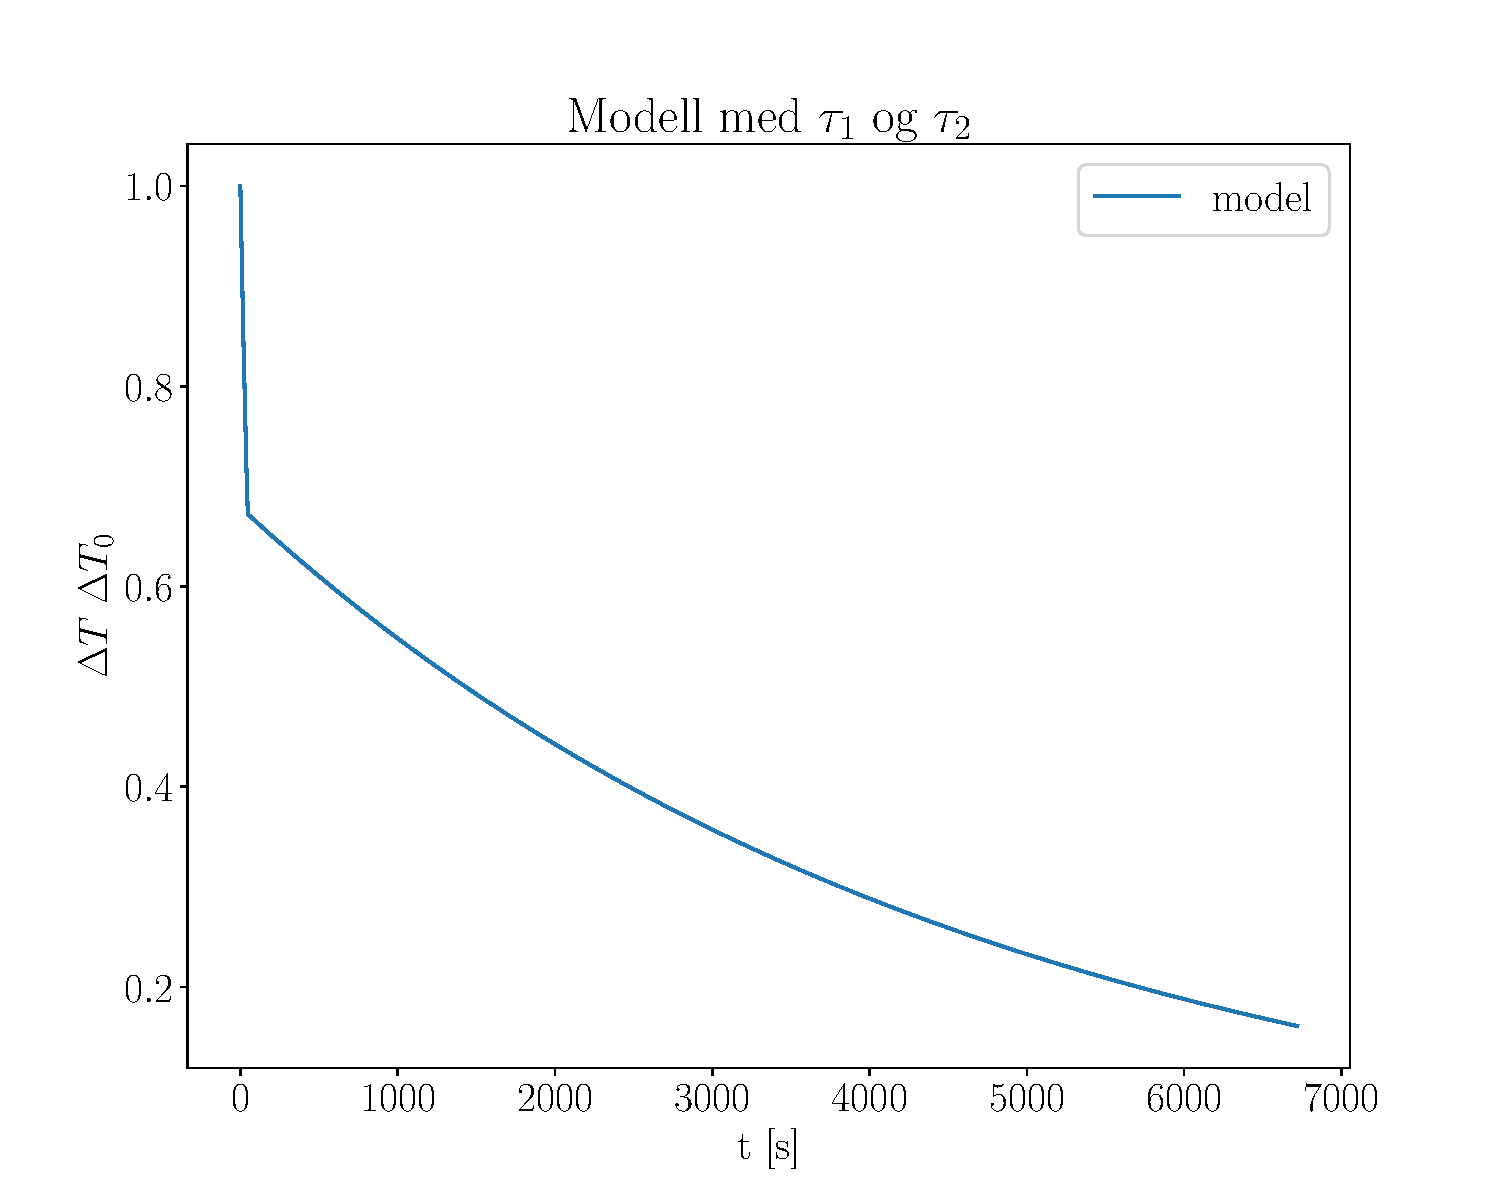
\includegraphics[scale=0.35]{2tauplot.pdf}
\caption{Skisse av hvordan den naive modellen for varmakapasitansforholdet vil se ut som en modell for 'Temperfect mug'.}
\label{plot2tau}
\end{figure}

Den modellen passer ikke så bra siden vi ikke har med den delen hvor temperaturkurven flater ut.

\subsection*{Sammenlign varmetapet til luften ved den normale koppen og tempperfect.}

Ser på forskjellen i temperatur, illustrert i \ref{tempdif}

\begin{figure}
\centering
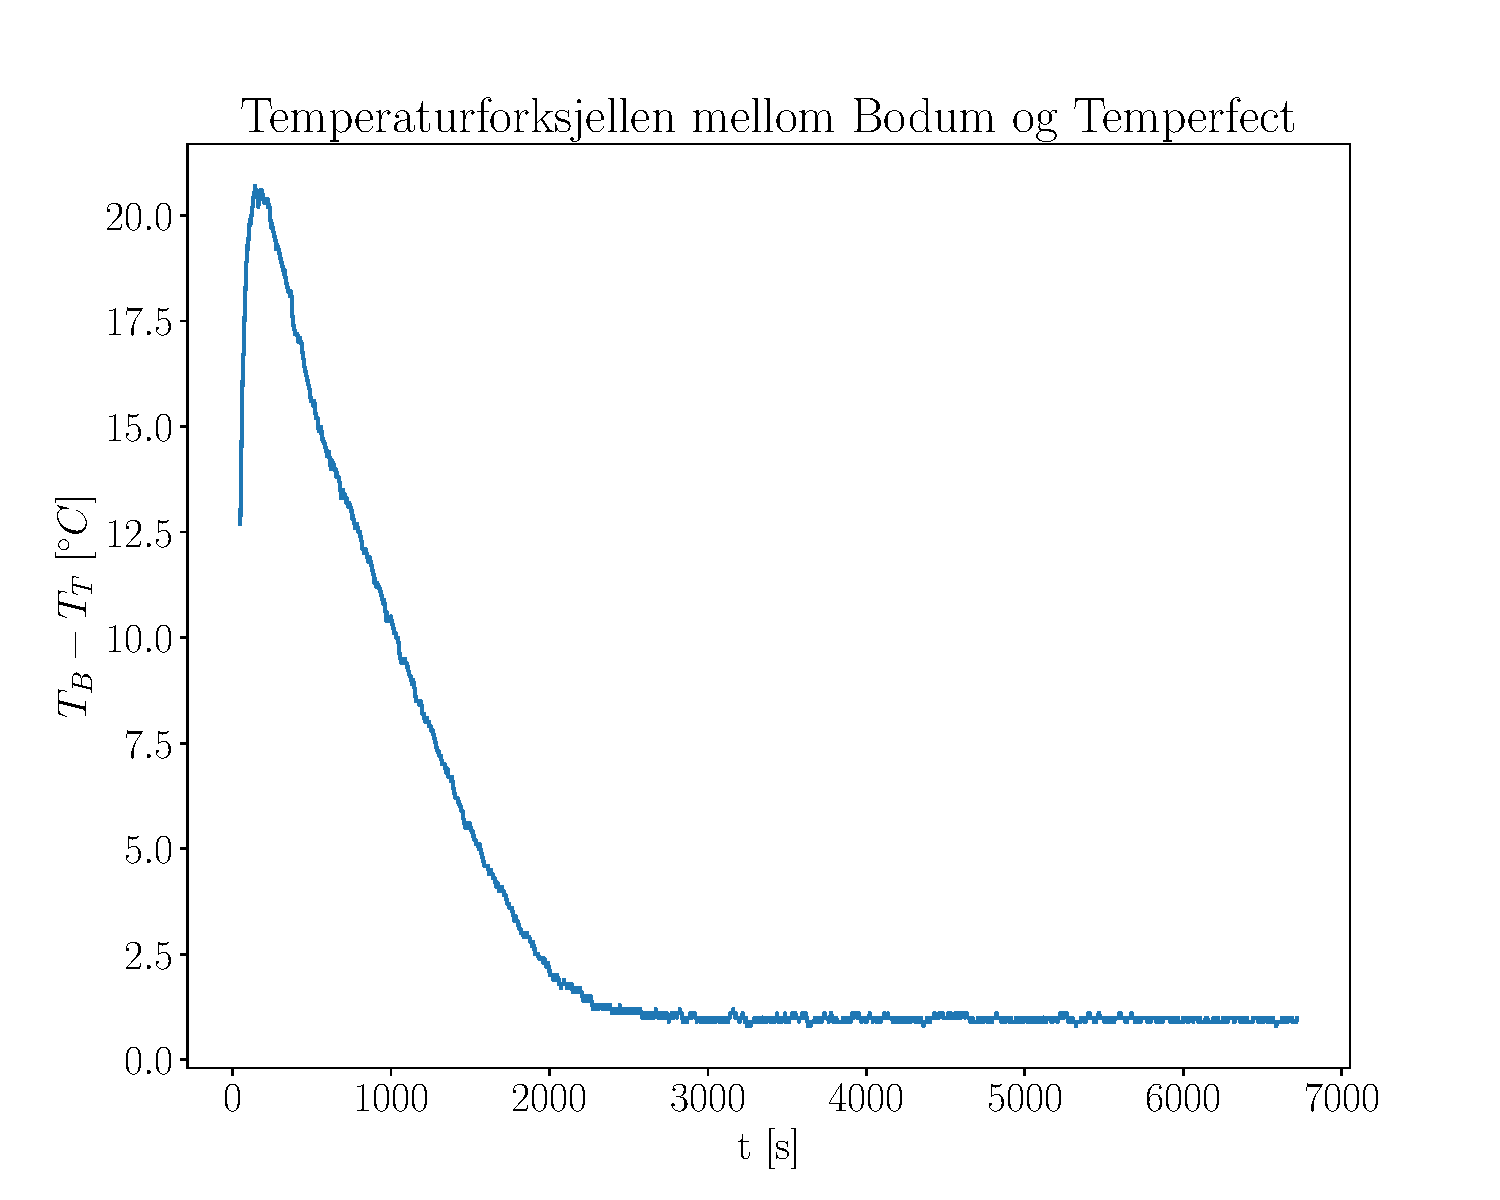
\includegraphics[scale=0.35]{tempzoomedout.pdf}
\caption{Temperaturforksjllen mellom Bodum-koppen og 'Temperfect mug'.}
\label{tempdif}
\end{figure}

Ser at den har en stor forskjell i starten, men så går de mer og mer like etter lengre tid.

\subsection*{Beregn multiplisiteten og entropien som en funksjon av q i en einstein krystal $(q, N)$}

Gjør bergningene og får følgende \ref{lavTS} og \ref{lavTC} for entropi og for varmekapasiteten.

\begin{figure}
\centering
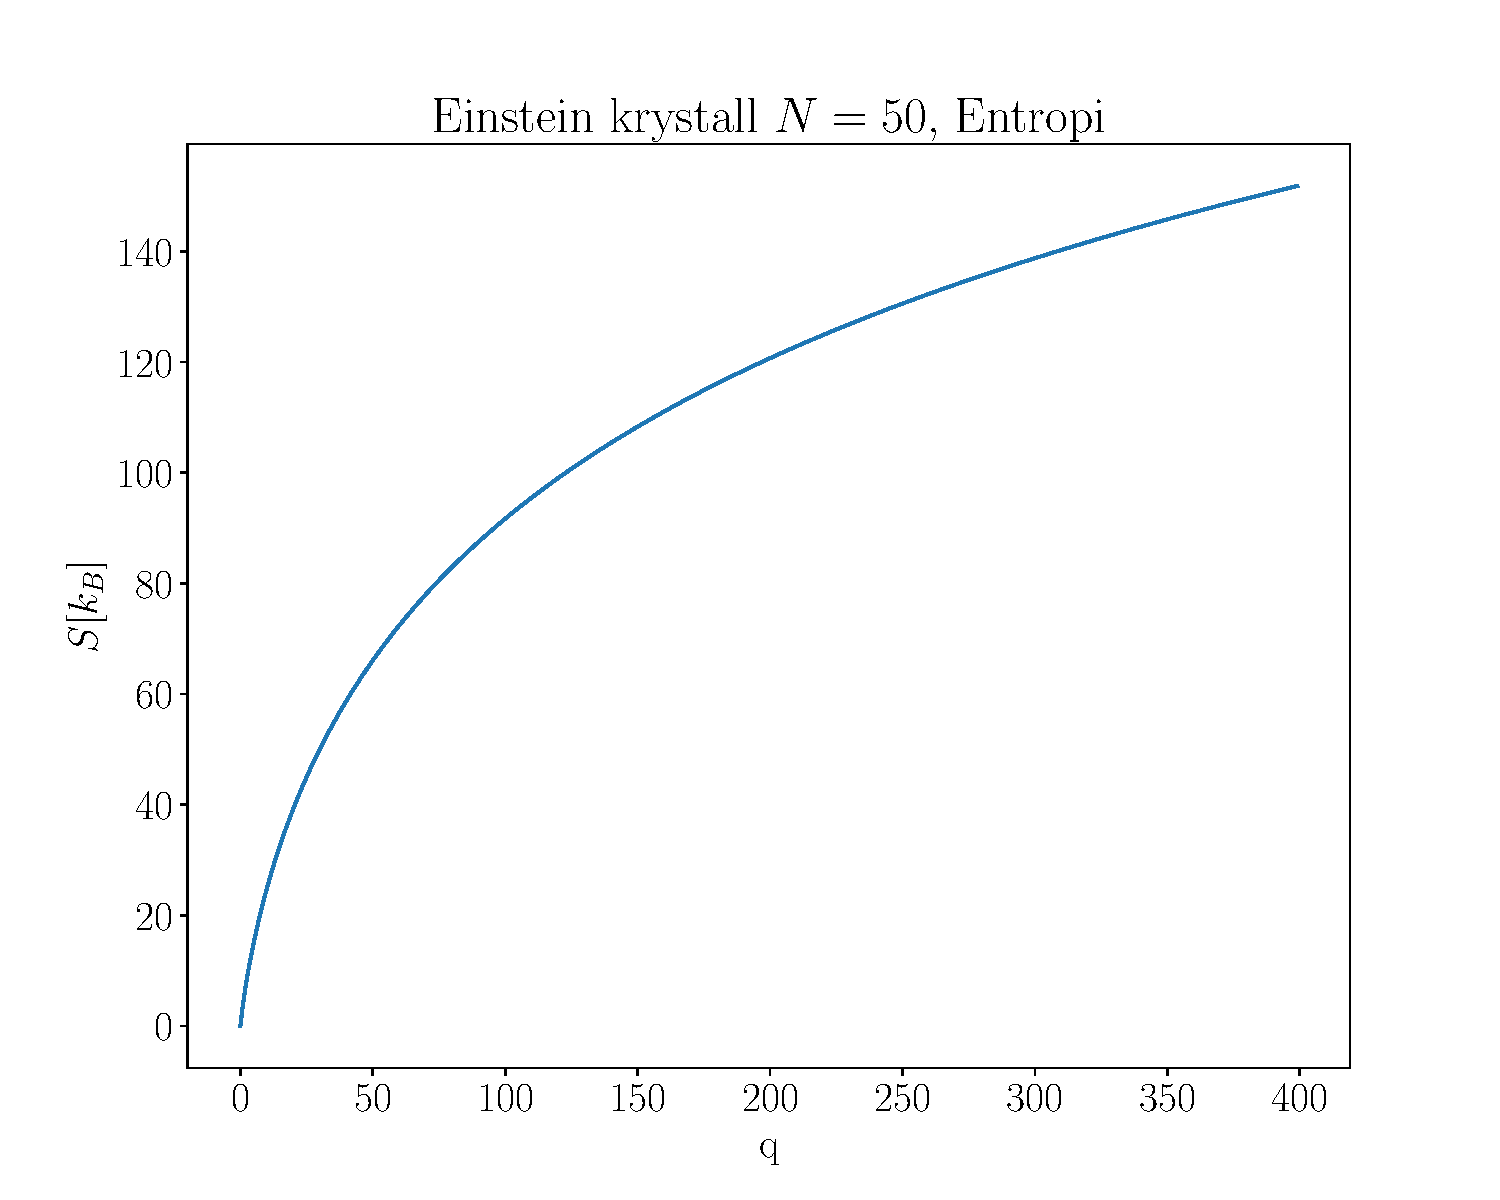
\includegraphics[scale=0.35]{lavTS.pdf}
\caption{Entropien til en einsteinkrystall. Entropien er i enhetene til boltzmannkonstant.}
\label{lavTS}
\end{figure}


\begin{figure}
\centering
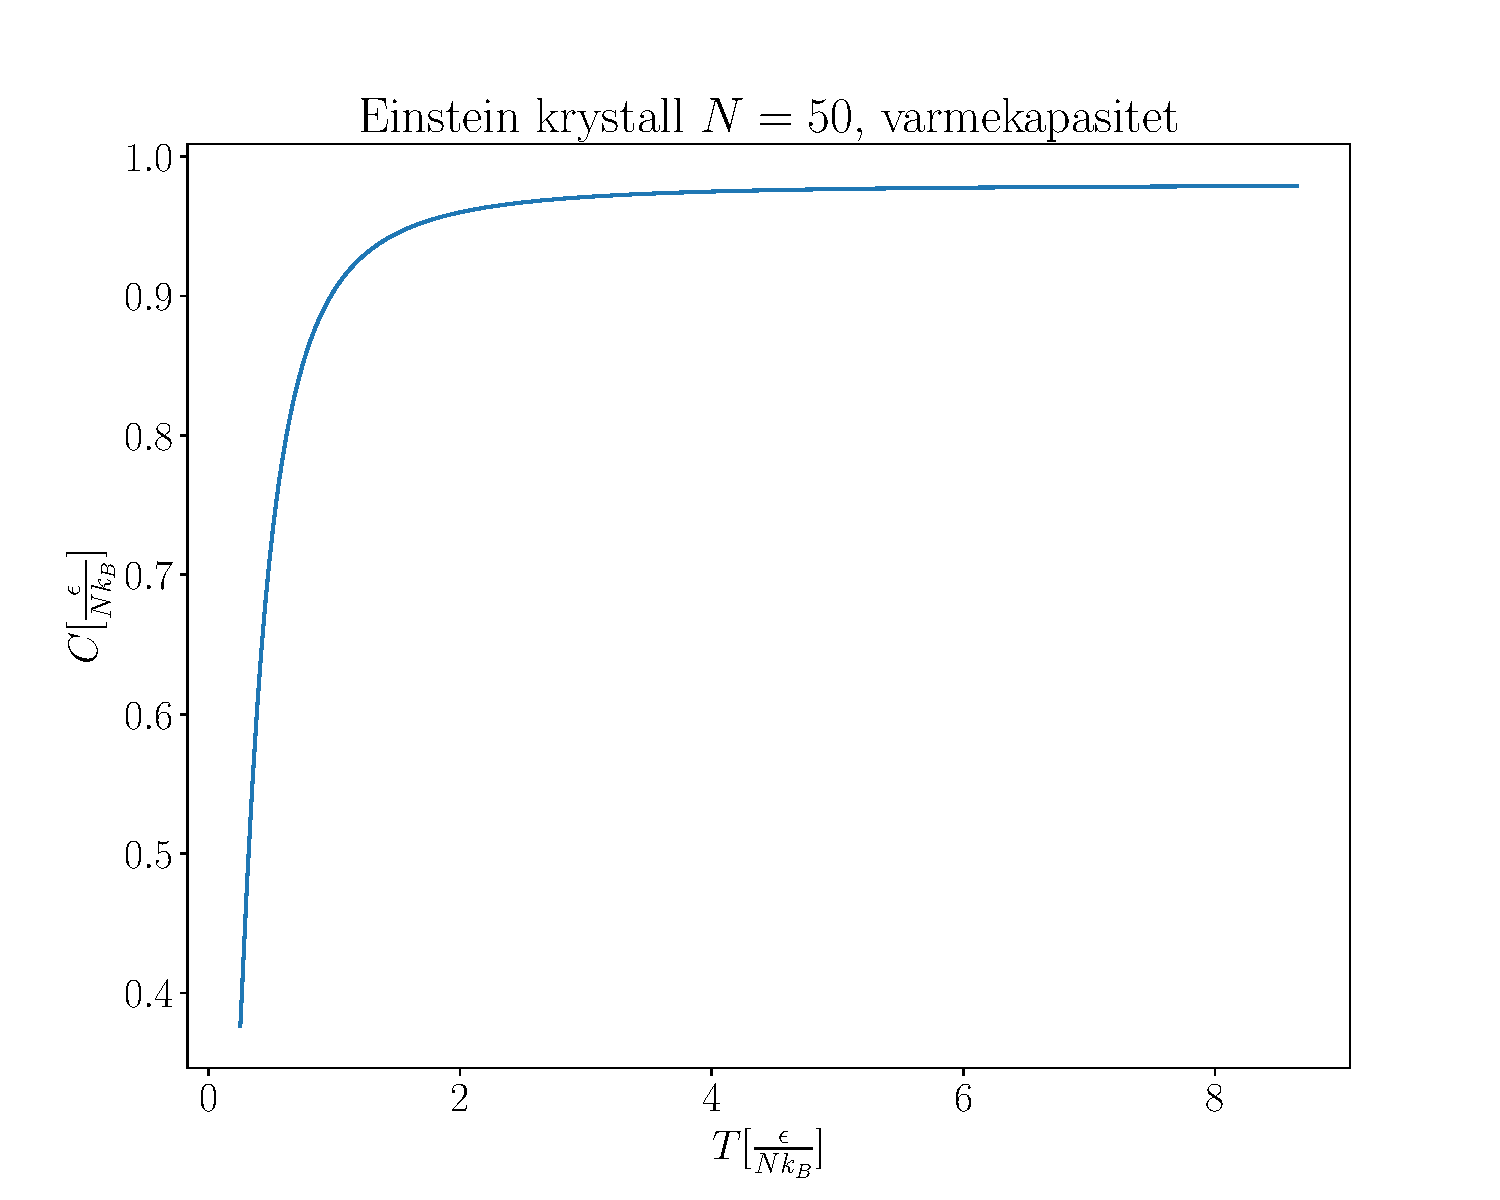
\includegraphics[scale=0.35]{lavTC.pdf}
\caption{Vamrekapasiteten til en einsteinkrystall. Kapasiteten er i enhetene til energien over boltzmannkonstanten og normalisert med antall oscilatorer.}
\label{lavTC}
\end{figure}


\subsection*{Vis utrykket for multiplisiteten til en einstseinkrystall analytisk}

Starter med utgangspunktet

$$ \Omega(q, N) = \frac{( q + N -1)!}{q!(N-1)!} $$

Som vi kan estimere for høye tall til å være nær

$$\approx \frac{( q + N)!}{q!N!}$$

Stirlings tilnærming sier oss at

$$n! \approx \sqrt{2\pi n} \left ( \frac{n}{e} \right ) ^n$$

Om vi neglesjerer kvadratrotfaktoren og skriver inn

$$\Omega \approx \frac{\left ( \frac{q+N}{e} \right ) ^{q+N}}{\left ( \frac{q}{e} \right ) ^q  \left ( \frac{N}{e} \right ) ^N} $$

Hvor kan omskrive til

$$\Omega \approx \frac{\left ( q+N \right ) ^{q+N} \left( \frac{1}{e} \right )^{q+N}}{ q^q   N^N \left( \frac{1}{e} \right )^{q+N}}$$

Og forkorte

$$\Omega \approx \frac{ \left ( q+N \right ) ^{q+N}}{q^q   N^N }$$

Som kan omskrives til
$$\Omega \approx \left ( \frac{q+N}{q}\right )^q \left ( \frac{q+N}{N}\right )^N$$

Dette utrykket stemmer overens med uttrykket for høye temperaturer ved at det er da man kan bruke Strilings aproksimasjon, for lave temperaturer så blir feilen for stor.

\subsection*{Finn det analytiske uttrykket for $S_N(q)$}

Starter med 

$$ S = k \ln{\Omega}$$

Som forenkelhetsskyld

$$ S = ln{\Omega}$$

Setter inn $\Omega$ tilnærmet med Stirlings aproksimasjon

$$ S = \ln{\left ( \frac{q+N}{q}\right )^q \left ( \frac{q+N}{N}\right )^N} $$

Slår sammen og omskriver

$$ S = \ln{\frac{ \left ( q+N \right ) ^{q+N}}{q^q   N^N }}$$

$$ S = (q+N)\ln{q+N} - q \ln{q} - N\ln{N}$$


\subsection*{Finn det analytiske uttrykket for $T(U)$}

Vi har definisjonen

$$ \frac{1}{T} = \frac{\partial S}{\partial U}$$

Vi har at

$$\frac{\partial U}{\partial q} = \epsilon$$
$$\partial U = \epsilon \partial q$$

Sett inn

$$\frac{1}{T} = \frac{\partial S}{\epsilon \partial q}$$
$$\frac{1}{T} = \frac{\ln{q+N} - \ln{q}}{\epsilon}$$

Vi snur om

$$T(q) = \frac{\epsilon}{\ln{\frac{q+N}{q}}}$$

\subsection*{Finn det analytiske uttrykket for $C_v(T)$}

Om vi ser bort i fra energien i grunntilstaden så har vi at 

$$U(T') = \frac{N}{e^{1/T'} -1}$$

Hvor $T' = \frac{T}{\epsilon k_B}$. Varmekapasiteten er definert

$$C_v = \frac{\partial U}{\partial T}$$

$$C_v(T') = \frac{e^{1/T'}}{(e^{1/T'} - 1)^2}$$

\subsubsection*{Sammenlikn de analytiske og numeriske resultatene}

Skisserer de analytiske uttrykkene i \ref{Sanalytisk} og \ref{Vanalytisk}.

\begin{figure}
\centering
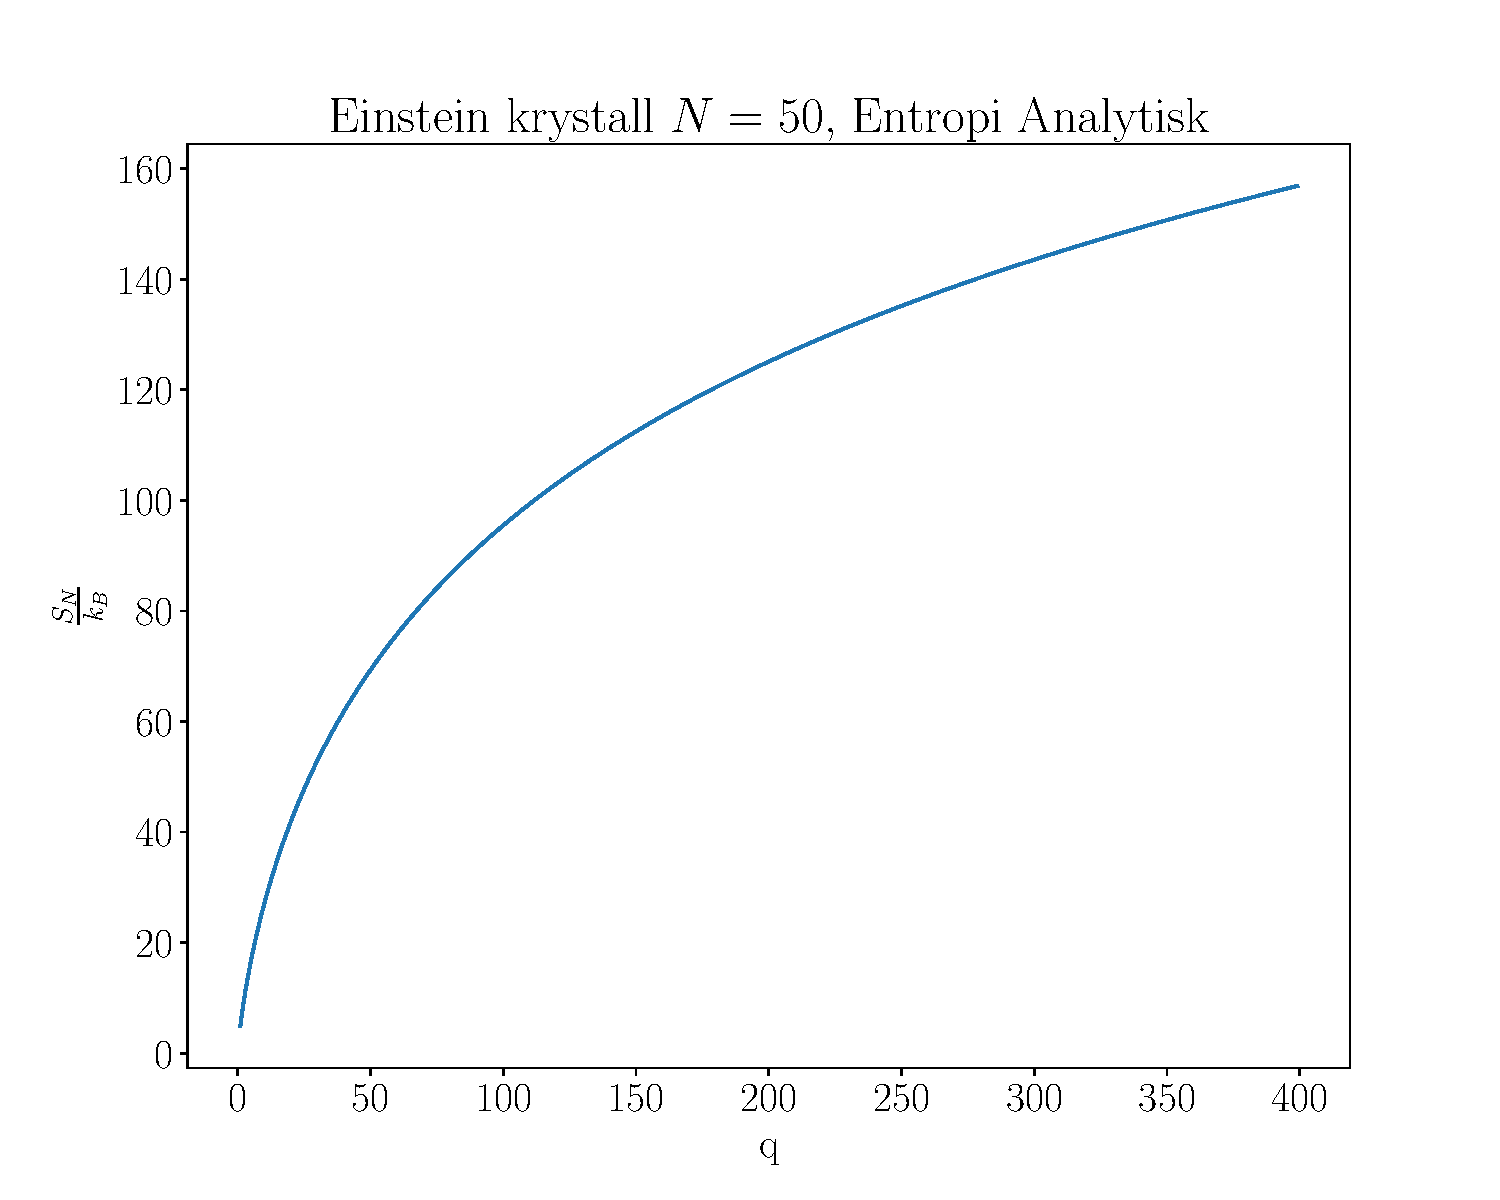
\includegraphics[scale=0.35]{Sanalytisk.pdf}
\caption{Den analytiske entropien for einsteinkrystall.}
\label{Sanalytisk}
\end{figure}


\begin{figure}
\centering
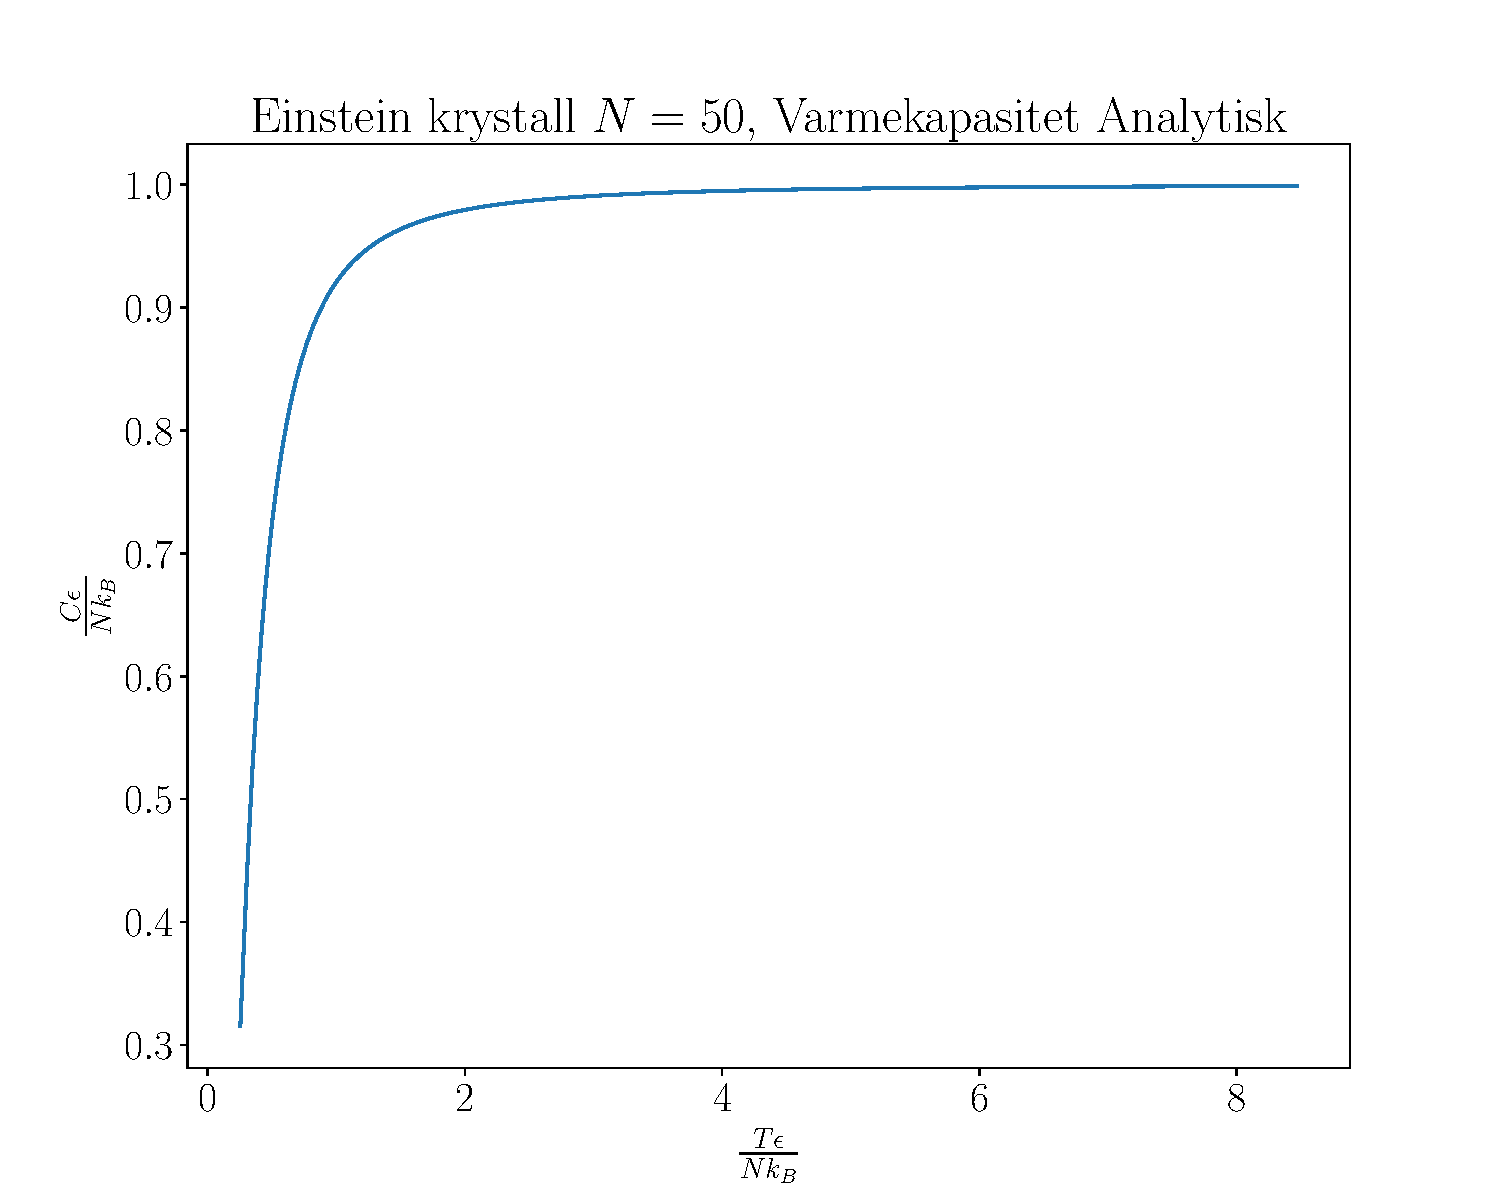
\includegraphics[scale=0.35]{Vanalytisk.pdf}
\caption{Den analytiske varmekapasiteten for einsteinkrystall.}
\label{Vanalytisk}
\end{figure}

Ser at de passer veldig bra overens. Med å se på Figur 1.14 i Schrõder så ser vi at vår modell har en 

$$\epsilon_{Pb} = 2k_B$$

$$\epsilon_{Al} = \frac{50}{23} k_B$$

$$\epsilon_{Diamond} = 5 k_B$$

\subsection*{Kan einstein krystall modellen bli brukt som en realitisk modell for 'Temperfect mug' sine viktige genskaper?}

Ja, ved å bruke uttrykket for varmekapasiteten avhengig av temperaturen så kan man få en modell som har en kontinuerlig endring av hvor mye kurven krummer. 

\section*{Konseptspørsmål}

\subsection*{Problem 1a}

Siden partikklene inne i thermosen blir presset tettere sammen så slår de mer på veggene som vil si at trykket øker.

\subsection*{Problem 1b}

Siden trykket øker så må temperaturen til gassen øke siden antall molekyler holdes konstant, og ingen varme kan slippe ut av systemet.

\subsection*{Problem 1c}

Når de trykkes sammen så vil molekylene ha mindre rom å bevege seg i som vil si at de vil ha flere kollisjoner med veggene. Arbeidet gjort på de  molekylene som var i den delen av volumet som ble presset vekk har fått en ekstra kinetisk energi som tilsvarer høyere temperatur. Den kinetiske energien vil fordeles raskt gjevnt utover hele gassen etterhvert som dmolekylene koliderer med hverandre. Den gjennomsnittlige kinetiske energien øker, som vil si at tempertauren øker.

\subsection*{Problem 1d}

Entropien øker siden temperaturen øker.

\subsection*{Problem 2a}

Nå vil kollisjonene med veggene av flasken ikke være fullstendig ellastisk, slik at den kinetiske energien de får fra sammenpressingen overføres til veggen så til omgivelsene rundt flasken. 

\subsection*{Problem 2b}

Selv om temperaturen holdes konstant, så øker trykket siden volumet blir mindre. 

\subsection*{2c}

De har samme gjennomsnitllig kinetisk energi, men mindre rom å bevege seg i, så de vil fortsatt kollidere med veggene oftere.

\subsection*{Problem 2d}

Vi har fortsatt endring i entropi, som vi kan se ved

$$\mathrm{d}U = T\mathrm{d}S - \rho \mathrm{d}V$$

Siden temperaturen hjolde konstant

$$\mathrm{d}S = \frac{\rho}{T}\mathrm{d}V$$

Siden vi har en forandring i volum så har vi en forandring i entropi, selv om vi holder temperaturen konstant innad i systemet.

\subsection*{Problem 3a}

Ja de har det. Siden de ligger i en struktur med tiltrekkningskrefter mellom molekylene som holder det sammen, så har de en større gjennomsnitsenergi. Den kjemiske energien er stor.

\subsection*{Problem 3b}

Siden de holdes sammen en tilrekkende krefter, så må det påføres en kraft for å fjerne de fra hverandre. Det vil si at det krever et negativt arbeid, altså vann-molekylene har mer negativ potensiell energi enn luft-molekylene. 

\subsection*{Problem 3c}

Ved samme temperatur, så har de like mye gjennomsnittlig kinetisk energi.

\subsection*{Problem 3d}

Hvor luft-molekylene beveger seg til de koliderer med et annet molekyl, så vil vann-molekylene vibrere i en kamp mot de intermolekylære kreftene .

\subsection*{Problem 3e}

Oppvarmingen av vannet vil kreve mer energi enn oppvarmingen av luft med samme volum. I begge tilfellene så vil molekylene får større kinetisk energi og bevege seg mer. 

\subsection*{Problem 3f}

Ihvertfall det ytterste laget av isen har samme temperatur som vannet som ligger het intill det. Når isen smelter så er det bevegelsen til molekylene blir for store til å opprettholde strukturen vannet trenger til å være et fast stoff. Den kinetiske energien som tilføres isen går til molekylene som så bruker det til å frigjøre seg fra noen av de tiltrekkende kreftende mellom molekylene, slik at når de er i flytende form så har de samme temperatur som når de var i fast form, ettersom den kinetiske energien er den samme.




\end{document}
